\documentclass{thesis-ekf}
\usepackage[T1]{fontenc}
\PassOptionsToPackage{defaults=hu-min}{magyar.ldf}
\usepackage[magyar]{babel}
\usepackage{amssymb,amsthm,pdfpages,listingsutf8,placeins}
\footnotestyle{rule=fourth}
\usepackage[dvipsnames]{xcolor}
\theoremstyle{definition}
%\newtheorem{definicio}[tetel]{Definíció}
\theoremstyle{remark}
\newtheorem{megjegyzes}{Megjegyzés}

\renewcommand\lstlistingname{Kódrészlet}

\lstdefinestyle{json}{
	backgroundcolor=\color{gray!20},
	stringstyle=\color{red},
	keywordstyle=\color{blue},
	keywordstyle=\color{purple},
	numbers=left,
	numberstyle=\tiny\color{gray},
	stepnumber=1,
	numbersep=5pt,
	showspaces=false,
	showstringspaces=false,
	showtabs=false,
	frame=single,
	rulecolor=\color{black},
	tabsize=2,
	breaklines=true,
	breakatwhitespace=true,
	captionpos=b
}
\lstdefinelanguage{Dart}{
	keywords={abstract, as, assert, async, await, break, case, catch, class, const, continue, covariant, default, deferred, do, dynamic, else, enum, export, extends, extension, external, factory, false, final, finally, for, Function, get, hide, if, implements, import, in, interface, is, library, mixin, new, null, on, operator, part, required, rethrow, return, set, show, static, super, switch, sync, this, throw, true, try, typedef, var, void, while, with, yield},
	keywordstyle=\color{blue}\bfseries,
	sensitive=true,
	comment=[l]{//},
	morecomment=[s]{/*}{*/},
	commentstyle=\color{gray}\ttfamily,
	string=[b]',
	morestring=[b]",
	morestring=[b]''',
	morestring=[b]""",
	stringstyle=\color{red}\ttfamily,
	numbers=left,
	numberstyle=\tiny\color{gray},
	stepnumber=1,
	numbersep=5pt,
	backgroundcolor=\color{white},
	showspaces=false,
	showstringspaces=false,
	showtabs=false,
	tabsize=2,
	breaklines=true,
	breakatwhitespace=true,
	captionpos=b,
	frame=single,
	rulecolor=\color{lightgray},
	basicstyle=\ttfamily\small,
	emph={int, double, num, String, bool, List, Map, Set, Runes, Symbol, dynamic, void},
	emphstyle=\color{purple}\bfseries,
	moredelim=[is][\color{orange}]{@}{@},
}
\lstdefinestyle{Dart}{
	breaklines=true,
}

\lstdefinestyle{JavaScript}{
	keywords={typeof, new, true, false, catch, function, return, null, catch, switch, var, if, in, while, do, else, case, break},
	keywordstyle=\color{blue}\bfseries,
	ndkeywords={class, export, boolean, throw, implements, import, this},
	ndkeywordstyle=\color{darkgray}\bfseries,
	identifierstyle=\color{black},
	sensitive=false,
	comment=[l]{//},
	morecomment=[s]{/*}{*/},
	commentstyle=\color{purple}\ttfamily,
	stringstyle=\color{red}\ttfamily,
	morestring=[b]',
	morestring=[b]"
	backgroundcolor=\color{gray!20},
	stringstyle=\color{red},
	keywordstyle=\color{blue},
	keywordstyle=\color{purple},
	numbers=left,
	numberstyle=\tiny\color{gray},
	stepnumber=1,
	numbersep=5pt,
	showspaces=false,
	showstringspaces=false,
	showtabs=false,
	frame=single,
	rulecolor=\color{black},
	tabsize=2,
	breaklines=true,
	breakatwhitespace=true,
	captionpos=b
}
\begin{document}
	
	\institute{Matematikai és Informatikai Intézet}
	\title{Moduláris Plug \& Play IoT / okos~otthon rendszer}
	\author{Farkas Levente\\Program tervező informatikus BSc}
	\supervisor{Dr. Geda Gábor\\egyetemi docens}
	\city{Eger}
	\date{2025}
	\maketitle
	\chapter*{Köszönetnyilvánítás}
	Szeretném kifejezni legmélyebb hálámat és őszinte köszönetemet konzulensemnek, Dr.~Geda Gábornak, aki szakmai hozzáértésével, segítőkészségével és türelmével végigkísért a szakdolgozat elkészítésének teljes folyamatán. Minden alkalommal számíthattam az iránymutatására, értékes tanácsaira és építő jellegű visszajelzéseire, amelyek nagyban hozzájárultak munkám színvonalához. Köszönöm, hogy mindig nyitott volt a kérdéseimre, és bátorított az önálló gondolkodásra.
	
	Külön köszönet illeti a családomat, akik végig támogattak tanulmányaim során. Nélkülük nem lett volna lehetséges eljutni idáig. Köszönöm a türelmüket, megértésüket, és azt a biztonságot és szeretetet, amelyet mindig érezhettem a háttérben. Ők jelentették számomra a stabil pontot minden nehezebb pillanatban.
	
	Hálás vagyok a barátaimnak is, akik nemcsak lelkileg támogattak, hanem gyakorlati segítséget is nyújtottak, amikor szükségem volt rá. Köszönöm a sok bátorítást, a motiváló beszélgetéseket, és hogy mindig tudtam, számíthatok rájuk.
	
	Végül köszönet illeti mindazokat, akik bármilyen formában hozzájárultak e dolgozat elkészültéhez – akár tudásmegosztással, inspirációval, akár csak egy jó szóval a megfelelő pillanatban.
	
	\tableofcontents
	\chapter*{Bevezetés}
	\addcontentsline{toc}{chapter}{Bevezetés}
	
	Az emberi civilizáció létezésétől kezdve a kényelemre törekedett. Minden nap valamivel könnyebbé, egyszerűbbé akarjuk tenni a mindennapokat, hogy minél kevesebbel kelljen foglalkoznunk és több időt tölthessünk más tevékenységgel. Az okos otthon rendszerek pontosan ezt teszik lehetővé, ezek régen drágák voltak így  a kevésbé tehetős emberek nem engedhették meg maguknak. Ma azonban olcsóbb ökoszisztémák is léteznek, de még így sem tudják sokan megfizetni. A projekt, amiről ezen dolgozat szól egy olcsóbb, közösség alapú, Apple szerű ökoszisztéma létrehozására törekszik, amely költséghatékonyabb megoldást kínál.
	
	Számomra lenyűgöző belegondolni abba, hogy pár sor kóddal ki tudunk hatni a környezetünkre. Főképp azért, mert a programozás szempontjából én mindig adatkezelésként tekintettem a munkánkra. Még a szakdolgozat témájának kiválasztása előtt kapcsolatba kerültem a mikrokontrollerek világával és attól a ponttól nem tudtam elengedni ezen eszközök varázsát. Tekintettel arra, hogy az áramkörök és elektromosság foglalkoztatott hobbi szinten már régóta, ez egy nagyszerű lehetőség volt, hogy kettő nagy szenvedélyemet, az informatikát és az áramköröket ötvözzem a szakdolgozatomban. Számomra hihetetlen volt akár csak egy LED\footnote{Light Emitting Diode, avagy fényt kibocsájtó dióda.} villanása is.
	
	Szakdolgozatom termék-orientált. Célja az, hogy a kevésbé tehetős emberek számára is elérhetővé tegye az okos otthonok varázsát. Általános tapasztalat szerint az okos eszközök árát nagyrészt a programozható mikrochipek teszik ki, ezeknek egy részről a hozzá tartozó áramkört kell vezérelniük, amely nem egy nehéz feladat, azonban az adatnak, amely alapján ez működni fog valahogy el kell jutnia az eszközhöz. Az elemek kapcsolata vezeték nélküli kapcsolattal valósul meg, amely minden esetben WiFi-n keresztül történik, azonban ez a fajta megközelítés jelentősen megemeli a hardver árát. Elképzelésem szerint a több különálló drága technológiát központosítani lehetne, amely az összköltség csökkenéséhez vezetne.
	
	Az eszköz önmagában nem képes sok mindenre, azonban a hozzá kapcsolódó ,,buta'' modulok használatával lehetőség nyílik arra, hogy egy eszköz négy modult, azaz működésében különálló okos eszközt kezeljen.
	A fejlesztés idejében az eszköz négy modult képes befogadni, azonban ez áramkör és program módosítással növelhető.
	
	Számomra fontos volt még az általam nem ismert, vagy nem használt technológiák használata, így próbáltam minél több számomra új technológiát használni, ezekről a technológiákról bővebben a \ref{ch_tech}.~fejezetben olvashatnak.
	\begin{center}
		Forráskód elérhetősége:\\
		{\color{blue}{\url{https://github.com/wolfino65/vy5sdy_thesis}}}
	\end{center}
	\chapter{Technológiai áttekintés}
	\label{ch_tech}
	\section{Eszköz oldalon alkalmazott technológiák}
	A rendszer sokrétű felépítése eredményeként több technológiát és programot fel kellet kutatnom, valamint ezek használatát minél jobban el kellett sajátítanom.
	\subsection{ESP programozásához használt nyelv}
	Ahogy később a \aref{ch_esp}.~fejezet \aref{se_espB}.~szekciójában olvasható az ESP32 eszközöket C/C++ nyelveken lehet főképp programozni, ezek mellett script nyelveket is lehet használni.
	
	A megoldásban első sorban C++ nyelvet akartam használni, azonban ez a megközelítés felvetett számos problémát a megvalósítás közben (ezekről bővebben a \aref{sub_fejlESP}.~alszekcióban olvashat). A problémák hatására célszerűnek találtam a C++ programozási nyelv leváltását, amelyet a MicroPython váltotta fel.
	
	A fejlesztés alapjául a programozási nyelv változásának eredményeként a  ESP32\_GENERIC\_S3-SPIRAM\_OCT-20241129-v1.24.1 firmware szolgált . Ami elérhető a \href{https://micropython.org/download/}{\color{blue}{MicroPython}} weboldalán.
	\subsection{Integrált fejlesztői környezet, IDE}
	\label{ssec_ide_esp}
	A fejlesztéshez választott fejlesztői környezet eredetileg a Visual Studio Code volt. -- azonban bármely extensiont próbáltam használni egyik sem tudta sikeresen feltölteni a programot az ESP-re -- Ennek eredményéül a fejlesztés első szakaszában a VSCode-ban megírt programot az Arduino IDE segítségével töltöttem fel.
	
	A programozási nyelv váltása után a VSCode továbbra sem volt működőképes, valamint az Arduino IDE nem támogatta a MicroPython nyelvet. Miután a probléma megoldására általam ismert módszerek tárháza kifogyott elkezdtem egy másik IDE után keresni. A keresésem eredményeként rátaláltam egy weboldalra\footnote{\url{https://randomnerdtutorials.com/micropython-ides-esp32-esp8266/}}, ahol több fejlesztői környezetet említenek. A keresés folyamatában számos GitHub és StackOverflow beszélgetést néztem át a válasz után kutatva. Ezekben a beszélgetésekben többször is említették a \href{https://thonny.org/}{\color{blue}{ThonyIDE}}-t. Ennek eredményéül kezdtem el használni az említett környezetet.
	\section{A REST API technológia háttere}
	Az alkalmazás kommunikációs rétegét egy REST API biztosította, amelyet Node.js platformon fejlesztettem Express.js keretrendszer segítségével. A választott technológiák lehetővé tették a gyors prototípuskészítést és a skálázható szerveroldali logika kialakítását.
	\subsection{Kulcstechnológiák és Döntések}
	\begin{enumerate}
		\item Node.js és Express.js
		\begin{itemize}
			\item A Node.js ideális volt aszinkron, eseményvezérelt architektúrájából eredően a párhuzamos kérések kezelésére.
			\item Express.js-re a gyors fejlesztési ciklus és egyszerű útvonalak kialakítása miatt esett a választás.
		\end{itemize}
		\item Adatcsere formátuma a JSON\footnote{JavaScript Object Notation} több okból is.
		\begin{itemize}
			\item Széles körben használt és elfogadott modern fejlesztői eszközökben.
			\item Könnyen értelmezhető ember és gép számára is.
			\item Alacsony adatmennyiségű, de strukturált információtovábbítást tesz lehetővé.
		\end{itemize}
	\end{enumerate}
	A bejövő HTTP kérések törzsében rejlő JSON adat feldolgozásának könnyítése érdekében a body-parser könyvtárat használtam.
	\subsection{REST API technológiai előnyei} 
		\begin{itemize}
			\item Platformfüggetlen. Az API-t bármely eszköz használhatja, legyen az beágyazott eszköz, vagy egy mobil applikáció.
			\item Teljesítmény. A Node.js által használt I/O műveletek nem blokkolók, így tökéletes az esetlegesen több ezer eszköz kéréseink fogadására.
		\end{itemize}
	
	
	\section{Adatbázis}
	A MongoDB egy nyílt forráskódú, dokumentumorientált NoSQL adatbázis, amelyet skálázható és nagy teljesítményű alkalmazások fejlesztésére terveztek. A hagyományos relációs adatbázisokkal (pl. MySQL, PostgreSQL) ellentétben a MongoDB nem táblákban, hanem rugalmas, JSON-szerű dokumentumokban tárolja az adatokat. Ez lehetővé teszi a gyors és hatékony adatkezelést, különösen olyan esetekben, amikor az adatok szerkezete dinamikus vagy változó.
	
	Fő jellemzői a MongoDB-nek:
	\begin{enumerate}
		\item Dokumentumorientált adatmodell:
		\begin{itemize}
			\item Az adatokat BSON (Binary JSON) formátumban tárolja, ami egy bináris reprezentációja a JSON-nek.
			\item Egy dokumentum egy kulcs-érték párokból álló struktúra, amely hasonlít a programozási nyelvekben használt objektumokhoz.
			\item Példa egy dokumentumra:\lstinputlisting[style=json,label=lst_docu,caption={Egy teszt dokumentum az adatbázisból.}]{docu.json}
		\end{itemize}
		\item Rugalmas séma:
		\begin{itemize}
			\item A MongoDB nem követeli meg, hogy minden dokumentumnak ugyanaz a szerkezete legyen. Ez lehetővé teszi, hogy különböző típusú adatokat tároljunk ugyanabban a gyűjteményben (collection).
			\item Például egy users gyűjteményben lehetnek olyan dokumentumok, amelyeknek nincs age mezője, vagy más mezők is lehetnek.
		\end{itemize}
		\item Skálázhatóság:
		\begin{itemize}
			\item A MongoDB horizontálisan skálázható, ami azt jelenti, hogy az adatbázis több szerverre (shard) osztható szét, hogy kezelni tudja a nagy mennyiségű adatot és a magas terhelést.
			\item Támogatja a replikációt is, ami magas rendelkezésre állást és hibaelállást biztosít.
		\end{itemize}
		\item Teljesítmény:
		\begin{itemize}
			\item A MongoDB gyors adatelérést biztosít indexek használatával. Többféle indexet támogat, beleértve az egyszerű, összetett, szöveges és geospatial indexeket.
			\item A memóriában történő adatkezelés (in-memory storage) tovább növeli a teljesítményt.
		\end{itemize}
		\item Aggregáció és lekérdezés:
		\begin{itemize}
			\item A MongoDB hatékony lekérdezési nyelvet (Query Language) és aggregációs keretrendszert (Aggregation Framework) biztosít az adatok elemzéséhez és feldolgozásához.
		\end{itemize}
	\end{enumerate}
	A MongoDB továbbá támogatja a CRUD műveleteket (Create, Read, Update, Delete), valamint a tranzakciókat is (a 4.0 verziótól kezdve).\cite{bib_mongo_sql}
	A MongoDB nem kényszeríti a sémák használatát, azonban van rá lehetőségünk, ha a feladat azt kívánja. A sémákban megadhatunk kötelező mezőket, azok típusát, valamint ezekhez köthetünk különböző ellenőrzéseket, úgynevezett validátor értékeket.
	\lstinputlisting[style=json,label=lst_schema,caption={Felhasználó collection sémája az adatbázisból. (A séma mezőinek azonosítója nem felelnek meg a json nyelv szabájainak, mivel a fájl tartalma konzolban került bevitelre.)}]{user_schema.json}
	
	Ahogy a \ref{lst_schema}.-es kódrészletben is látható típus és mező megszorításokat tartalmaz a séma, e mellett az email mező még reguláris kifejezéssel is vizsgálva van.
	\subsection{MongoDB struktúrája}
	A MongoDB az adatbázison belül táblák helyett collection-ök vannak, ezen belül rekordok, avagy sorokkal ellentétben dokumentumokat találunk, ahol oszlopok helyett mezők vannak. Az összehasonlítást egy hagyományos SQL adatbázissal a \ref{img_sql_mongo}.~ábrán lehet látni. \cite{bib_mongo_sql}
	 \begin{figure}[!h]
	 	\centering
	 	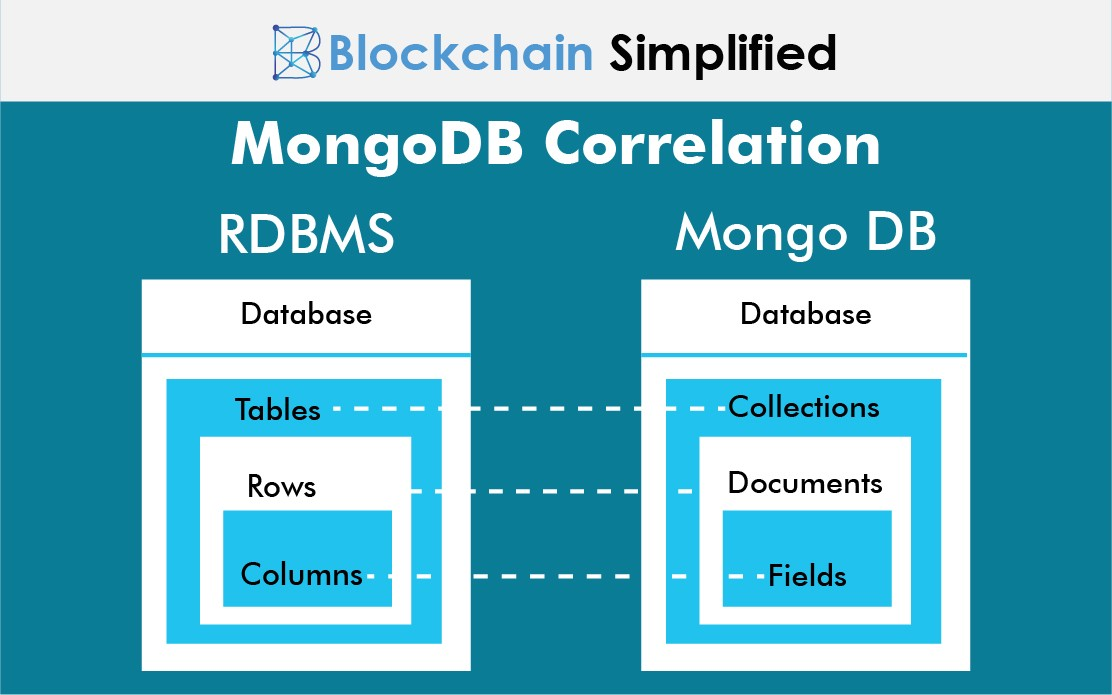
\includegraphics[width=8cm]{mongo_vs_sql}
	 	\caption{SQL adatbázis és MongoDB szerkezeti hasonlóságai.\cite{bib_mongo_sql}}
	 	\label{img_sql_mongo}
	 \end{figure}
	\section{Frontend technológia}
	Az eszköz hatékony vezéréléséhez szükségünk van egy applikációhoz, azonban lehet, hogy egyes emberek nem mindenhez a telefonjukat akarják használni. Ez problémát vet fel, mivel több kódbázis fenntartása és javítása sok embert és erőforrást igényel. 
	
	Megoldásként egy olyan keretrendszerre, vagy programozási nyelvre van szükség, amely működőképes több platformon is.
	
	\textbf{Például:}
	\begin{itemize}
		\item React Native
		\item Kotlin
		\item Flutter
		\item Lynx
	\end{itemize}
	\begin{megjegyzes}
		A legújabb keretrendszer a LynxJs, amely 2025.03.05.-én jelent meg. Ahogy a React Native ez is javascript alapú, így a Lynx és React Native egyfajta versenyhelyzetben vannak. A keretrendzerek összehasonlítását olvashatja a  \href{https://medium.com/@mostsignificant/introducing-lynx-how-tiktoks-new-framework-compares-to-react-native-580a52d3462c}{\color{blue}{Medium.com}}-on, valamint a \href{https://lynxjs.org/}{\color{blue}{LynxJs.org}}-on tudhat meg többet a keretrendszerről.
	\end{megjegyzes}
	
	React Native-ról meglehetősen sok negatív megjegyzést hallottam, miszerint rendkívül nehéz a használata és rengeteg nehezen javítható problémát eredményez, ha nem tökéletesen használjuk. Ismeretségi körömbe tartozik egy személy, aki arra esküdött fel, hogy soha többé nem fogja használni a túlságosan komplikált fejlesztés eredményeként.
	A Lynx tekintve, hogy rendkívül új, nagy valószínűséggel több, még rejtett hibákat tartalmazhat, valamint a dokumentáción kívül logikám szerint rendkívül alacsony a jelenleg elérhető egyéb források száma.
	A Kotlin, mint a Java helyettesítője alapvetően egy JVM\footnote{Java Virtual Machine}-et használ a program futtatására, amely nem optimális teljesítményhez vezethet. A probléma megoldására létrejött a Kotlin Native\cite{bib_kotlin_native_home}, azonban rendkívül lassú a JRE\footnote{Java Runtime Environment} verzióhoz képest, valamint nem létezik hozzá sok alapvető csomag, vagy ,,könyvtár''\cite{bib_kotlin_native_discussion}.
	A fent említett okok miatt, valamint a tény, hogy a Flutter natívan futó programot állít elő miatt választásom a Flutter-re esett.
	\subsection{Miért Flutter?}
	\begin{itemize}
		\item Könnyű crossplatform build lehetőség
		\item Opensource
		\item Gyorsaság\footnote{,,Flutter is powered by Dart, a language optimized for fast apps on any platform''\cite{bib_flutter_web}}
		\item Új technológia megismerése
		\item Native build-ek
	\end{itemize}
	A Flutter ezen tulajdonságai rendkívül kedvezővé tette a frontend applikáció elkészítéséhez. 
	\subsection{Flutter ismertetése}
	A Flutter egy olyan eszköz, amely lehetővé teszi a fejlesztők számára, hogy natív, többplatformos alkalmazásokat hozzanak létre egyetlen programozási nyelv és egyetlen kódbázis segítségével. Nem olyan alkalmazást hoz létre, amely böngészőben fut, vagy amelyet natív alkalmazásokba csomagolnak. Ehelyett natív alkalmazásokat készít iOS-re és Androidra is, amelyek később közzétehetők az app store-okban.
	
	
	Az alkalmazást létrehozásához egyetlen programozási nyelvre van szükségünk, ahelyett, hogy különböző nyelveket használnánk egy iOS vagy Android alkalmazás fejlesztéséhez. Így csak egyetlen kódbázissal kell foglalkoznunk. A Flutter egy SDK\footnote{Software Development Kit}, amely lehetővé teszi, hogy a kódbázisodat natív gépi kódra fordítsd, amely a fent említett platformokon fut.
	
	
	A fordítási eszközök mellett a Flutter keretrendszerként is funkcionál, UI építőelemeket (widgeteket) biztosít, mint például lapok, legördülő menük, gombok stb., valamint néhány segédfüggvényt és csomagot, amelyeket az SDK segítségével lehet lefordítani.\cite{bib_flutter_short}
	
	Flutter applikációt a fent említettek mellett még Windows-on, Linux-on és Web-en is lehet használni.
	\chapter{Rendszerterv}
	\label{ch_rendszert}
	\section{Rendszer célja}
	A szakdolgozat célja egy moduláris okos otthon rendszer fejlesztése, ahol egy köztes API-val van kapcsolatban minden eszköz. Az eszközöket két csoportba lehet sorolni. Célja egy community alapú rendszer kialakítása, ahol bárki fejleszthet különböző céllal modulokat a rendszerhez. Ez a megközelítés törekszik arra, hogy a rendszer összköltsége alacsony maradjon.
	\section{Architekturális terv}
	A rendszer 3 különböző projektből épül fel: multiplatform felhasználói felület (Flutter), moduláris eszköz (MicroPython, ESP32), valamint, amely ezt a kettő projektet összeköti a REST API (Node.js, Express.js). Tekintve, hogy egyik projektben használt programozási nyelv sem azonos, szükség van egy közös ,,nyelvre''. Ez a nyelv a JSON.
	\begin{itemize}
		\item \textbf{Multiplatform felhasználói felület}: Ez a felület szolgál a parancsok, avagy feladatok kiadására, amelyet a moduláris eszköz el fog végezni. Amennyiben csoportként tekintünk az egyes projektekre, ez a csoport a vezérlő csoport.
		\item \textbf{Moduláris eszköz}: Szerepe és munkája a felület által létrehozott feladatok ellátása és végrehajtása. Csoport szemléletben ez a végrehajtó csoport.
		\item \textbf{REST API}: A két csoport összekötésére hívatott köztes rendszer, amely lehetővé teszi a kommunikációt a csoportok között.
	\end{itemize}
	\section{Követelmények}
	\label{sec_kovetelmenyek}
	A szekció a fejlesztés sikeréhez szükséges követelményeket tartalmazza részletesen.
	\subsection{Felhasználói felület}
	A felület rendelkezik egy regisztrációs és bejelentkező oldallal, a kettő oldal eléréséhez nem szükséges semmilyen előzetes vizsgálat. A bejelentkező felület fogadja a felhasználót alapértelmezetten.
	Amennyiben a felhasználó engedélyt ad az automatikus bejelentkezéshez, a felhasználót az alapértelmezett felületet felülíró felület fogadja, amely a felhasználóhoz csatlakoztatott eszközök listáját tartalmazza.
	
	Az eszközök oldalon, amely a felülírja a bejelentkezés oldalt, találhatónak kell lennie egy gombnak, amellyel új eszközöket adhatunk hozzá. Mind e mellett ideálisan a jobb felső sarokban meg kell adni a felhasználónak a kijelentkezés lehetőségét és a saját adatainak változtatását. A listázott eszközök egyikére kattintva az eszköz moduljainak meg kell jelennie, valamint a felhasználónak lehetőséget kell adni az eszközhöz új modult csatlakoztatni, azt leválasztani és az eszköz adatainak változtatását lehetségessé tenni.
	
	Az eszköz opcióin belül több lehetőséget is figyelembe kell venni.
	\begin{itemize}
		\item Eszköz adatainak módosítása.
		\item Eszköz törlése.
		\item Eszköz opciói.
		\begin{itemize}
			\item Modul eltávolítása.
			\item Eszköz hálózatának alaphelyzetbe állítása.
			\item Eszköz moduljainak alaphelyzetbe állítása, amely az összes modult le kell csatlakoztatnia.
		\end{itemize}
	\end{itemize}
	
	A felhasználónak a beállításokon belül meg kell adni a lehetőséget a
	\begin{enumerate}
		\item automatikus bejelentkezés letiltására,
		\item felhasználónév cseréjére,
		\item jelszó cseréjére,
		\item e-mail cím módosítására
		\item és fiók törlésére.
	\end{enumerate}
	A fiók törlését, jelszó cseréjét és e-mail cím módosítását követően felületnek kötelezően vissza kell térnie a bejelentkezéshez használt oldalhoz. Ennek a műveletnek bármely felsorolt esetnél meg kell történnie.
	
	Az eszköz oldalnak tartalmazni kell 4 ,,csempét'', amely kattintással átvisz a modulhoz tartozó feladat paramétereit megadó oldalra. Fontos, hogy a moduláris állapot fenntartásának érdekében ezek az oldalak dinamikusan jelenjenek meg és az egyes modulokhoz legyenek párosítva. 
	\subsection{Eszköz követelményei}
	Az eszköznek képesnek kell lennie legalább 4 modul fogadására és azoktól függetlenül kell működnie.
	A felhasználó kizárólagosan az eszköz
	\begin{itemize}
		\item telepítésénél,
		\item konfigurálásánál,
	\end{itemize}
	valamint egyes modulok
	\begin{itemize}
		\item csatlakoztatásánál,
		\item leválasztásánál
	\end{itemize}
	szabad közvetlen kapcsolatba lépnie az eszközzel.
	
	Az eszköz konfigurálása WiFi-n keresztül kell történnie, valamint csatlakoznia kell az internethez. Az adatokat JSON formátumban kell feldolgoznia. Csatlakoztatás esetén kizárólagosan a csatlakozandó modult kell a felhasználónak megadnia, valamint leválasztás alkalmával nem kell semmit megadnia, azaz az eszköznek kell kezelnie, hogy melyik porthoz csatlakozott a modul. Ezeket a változásokat továbbá köteles megjeleníteni a az adatbázisban.
	
	Az eszköznek a beérkezett feladatról azonnal információt kell kapnia.
	\subsection{API, összekötő réteg követelményei}
	Az API köteles az összes táblára, vagy azzal egyen értékű szerkezethez kötődő műveletek megvalósítására. Azaz képes legyen ellátni azon szerkezet tartalmának műveleteit, mint egység az olvasása, létrehozása, frissítése, valamint törlése. Ezek mellett köteles egy modern, skálázható, könnyen kezelhető adatbázissal kapcsolatot létesítenie, amelyeken a fent említett műveleteket elvégezheti.
	\section{Alkalmazott fejlesztői eszközök}
	A rendszer fejlesztésének és üzemeltetésének folyamatát számos eszköz segítette elő.
	\subsection{Visual Studio Code}
	A Visual Studio Code (VS Code) egy modern, nyílt forráskódú kódszerkesztő, amelyet a Microsoft fejlesztett és 2015-ben adott ki. Azóta az egyik legnépszerűbb fejlesztői eszközzé vált, köszönhetően gyorsaságának, rugalmasságának és a gazdag funkcionalitásnak. Ingyenesen használható, és támogatja a Windows, macOS és Linux operációs rendszereket is, így széles körben elterjedt a fejlesztők körében.
	
	A VS Code nem csupán egy egyszerű szövegszerkesztő, hanem egy teljes értékű fejlesztői környezet, amely intelligens kódkiegészítéssel (IntelliSense), beépített Git-kezeléssel és hatékony hibakereső eszközökkel rendelkezik. A szerkesztő testreszabható felülete lehetővé teszi a témák, billentyűparancsok és bővítmények segítségével, hogy minden fejlesztő a saját igényeihez igazítsa.
	
	A bővítmények (extensions) rendszere hatalmas lehetőséget kínál a funkcionalitás bővítésére, legyen szó webfejlesztésről, adatbázis-kezelésről vagy akár mesterséges intelligenciával kapcsolatos eszközökről. Emiatt a VS Code nem csak kezdők, hanem professzionális fejlesztők számára is nélkülözhetetlen segédeszköz.
	
	A szoftver aktív fejlesztése és a közösség által támogatott nyílt forráskódú modell biztosítja, hogy folyamatosan fejlődik, új funkciókkal és optimalizálásokkal gazdagodva\cite{bib_vscode}.
	\subsection{Thonny IDE}
	A Thonny egy felhasználóbarát integrált fejlesztői környezet (IDE), amelyet elsősorban Python programozás tanítására és tanulására terveztek, különös hangsúllyal a MicroPython támogatásán. Az Észtországi \href{https://ut.ee/en}{\color{blue}{Tartu Egyetem}} fejleszti, és ingyenesen elérhető Windows, macOS és Linux platformokra.
	
	Ez az IDE kifejezetten kezdők számára készült, de a MicroPython támogatás miatt népszerű választás az embedded fejlesztésben is, különösen olyan mikrovezérlős projekteknél, mint az ESP32, ESP8266 vagy Raspberry Pi Pico. A Thonny beépített Python 3 és MicroPython interpretterrel rendelkezik, így nem igényel külön konfigurálást - ez ideális megoldást kínál mind a kódolás alapjainak elsajátításához, mind a fizikai számítógépes projektek fejlesztéséhez.
	
	A program egyik legnagyobb előnye a lépésről-lépésre történő kódvégrehajtás és a változók valós idejű vizualizációja, ami segít megérteni a program működését. MicroPython fejlesztéskor a Thonny lehetővé teszi a kód direkt feltöltését a mikrovezérlőre, valamint interaktív REPL (Read-Eval-Print Loop) konzolt biztosít a hibakereséshez.
	
	Bár a Thonny nem a legfejlettebb IDE összetett projektekhez, kiváló választás kezdőknek, oktatási célokra és egyszerűbb MicroPython-alapú fejlesztésekhez. Nyílt forráskódú termék, ami aktív fejlesztést és közösségi támogatást biztosít\cite{bib_thonny,bib_thonny_deepseek}.
	
	A Thonny IDE választásáról többet olvashat a \ref{ssec_ide_esp}.~szekcióban.
	\subsection{Git, Github}
	A Git egy nyílt forráskódú, verziókezelő rendszer, amely segítségével nyomonkövethető a projekt forráskódjai és fájljai, valamint azok változásai. A GitHub egy Git-re épülő népszerű online platform, amely lehetővé teszi távoli tárolók, úgynevezett repozitóriumok létrehozását és használatát. A GitHub projekt része lehetővé teszi, hogy a repozitóriumhoz csatoljunk úgynevezett projekteket, amely segítségével akár a Trello is helyettesíthető. A fejlesztés folyamán én a GitHub projekt részét használtam. A projektről készült képernyőkép megtekinthető a \ref{img_git}.~képen.
	\begin{figure}[!ht]
		\centering
		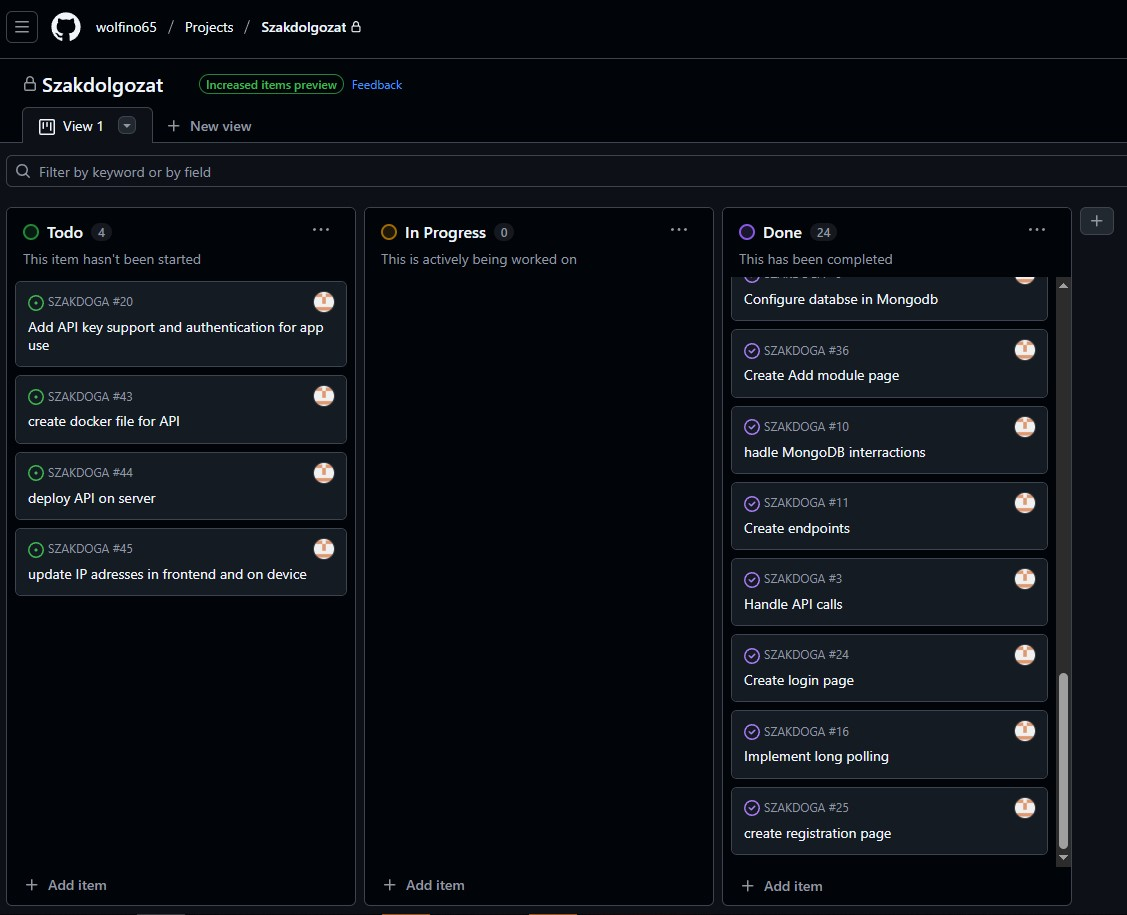
\includegraphics[width=15cm]{github_project}
		\caption{Szakdolgozathoz feladatkövetéshez használt GitHub projekt, és állapota [2025.04.10.]}
		\label{img_git}
	\end{figure}
	\subsection{További eszközök szerepe a fejlesztés folyamatában}
	\begin{itemize}
		\item \textbf{MongoDB Compass}: Grafikus felületet nyújtó program az adatbázis könnyű kezeléséhez.
		\item \textbf{Postman}: API teszteléshez használt eszköz.
	\end{itemize}
	\chapter{Az ESP32 mikrovezérlő bemutatása}
	\label{ch_esp}
	A projekt kulcsfontosságú része, maga az eszköz, amely lehetővé teszi a modulok vezérlését. A \ref{img_myesp}-es ábrán látható mikrokontrollerhez hasonlót több gyártó is gyárt, azonban egy ESP kifejezetten a benne található processzortól lesz ESP. Az ESP32-ben található Xtensa LX6 processzor két maggal van ellátva és órajele 240 MHz\footnote{Megahertz}.
	\section{ESP32 hardverének és fejlesztői környezetének bemutatása}
	\label{se_espB}
	Az ESP32 egy rendkívül sokoldalú és hatékony mikrokontroller, amely számos területen alkalmazható. Két magos processzora, integrált WiFi és Bluetooth képességei, valamint gazdag I/O lehetőségei miatt kiváló választás mind IoT, mind ipari vagy okos otthon alkalmazásokhoz. Az ESP32 fejlesztése egyszerű és gyors, köszönhetően a széles körben elérhető fejlesztői eszközöknek és könyvtáraknak. Ezek a tulajdonságok teszik az ESP32-t az egyik legnépszerűbb mikrokontrollerré a beágyazott rendszerek világában. Mind e mellett az általam választott változat nem szenved RAM, vagy ROM hiányában sem. Az adatlap szerint el van látva 512 KB SPRAM-al, 384 KB ROM-al és változó méretű PSRAM\footnote{Pseudo SRAM}-al. Az utóbbi a használt eszköz esetében 8 Mb, valamint még fel van szerelve 32MB Octal Flash\footnote{Az Octal (xSPI) Flash memória egy gyors memória típus, amely kedvelt beültetett rendszerek között, nagyrészt a memóriáról történő gyors boot-nak köszönhetően. A memória típus 400MB/s olvasási sebességre képes.\cite{bib_esp_octal}} memóriával.
	
	
	Az általam \aref{img_myesp} használt modell az ESP32-S3-DevKitC-1 N32R8V, amely egy ESP32-S3-WROOM-2 chipet tartalmaz, ezt az Espressif System fejlesztette ki.
	\begin{figure}[!ht]
		\centering
		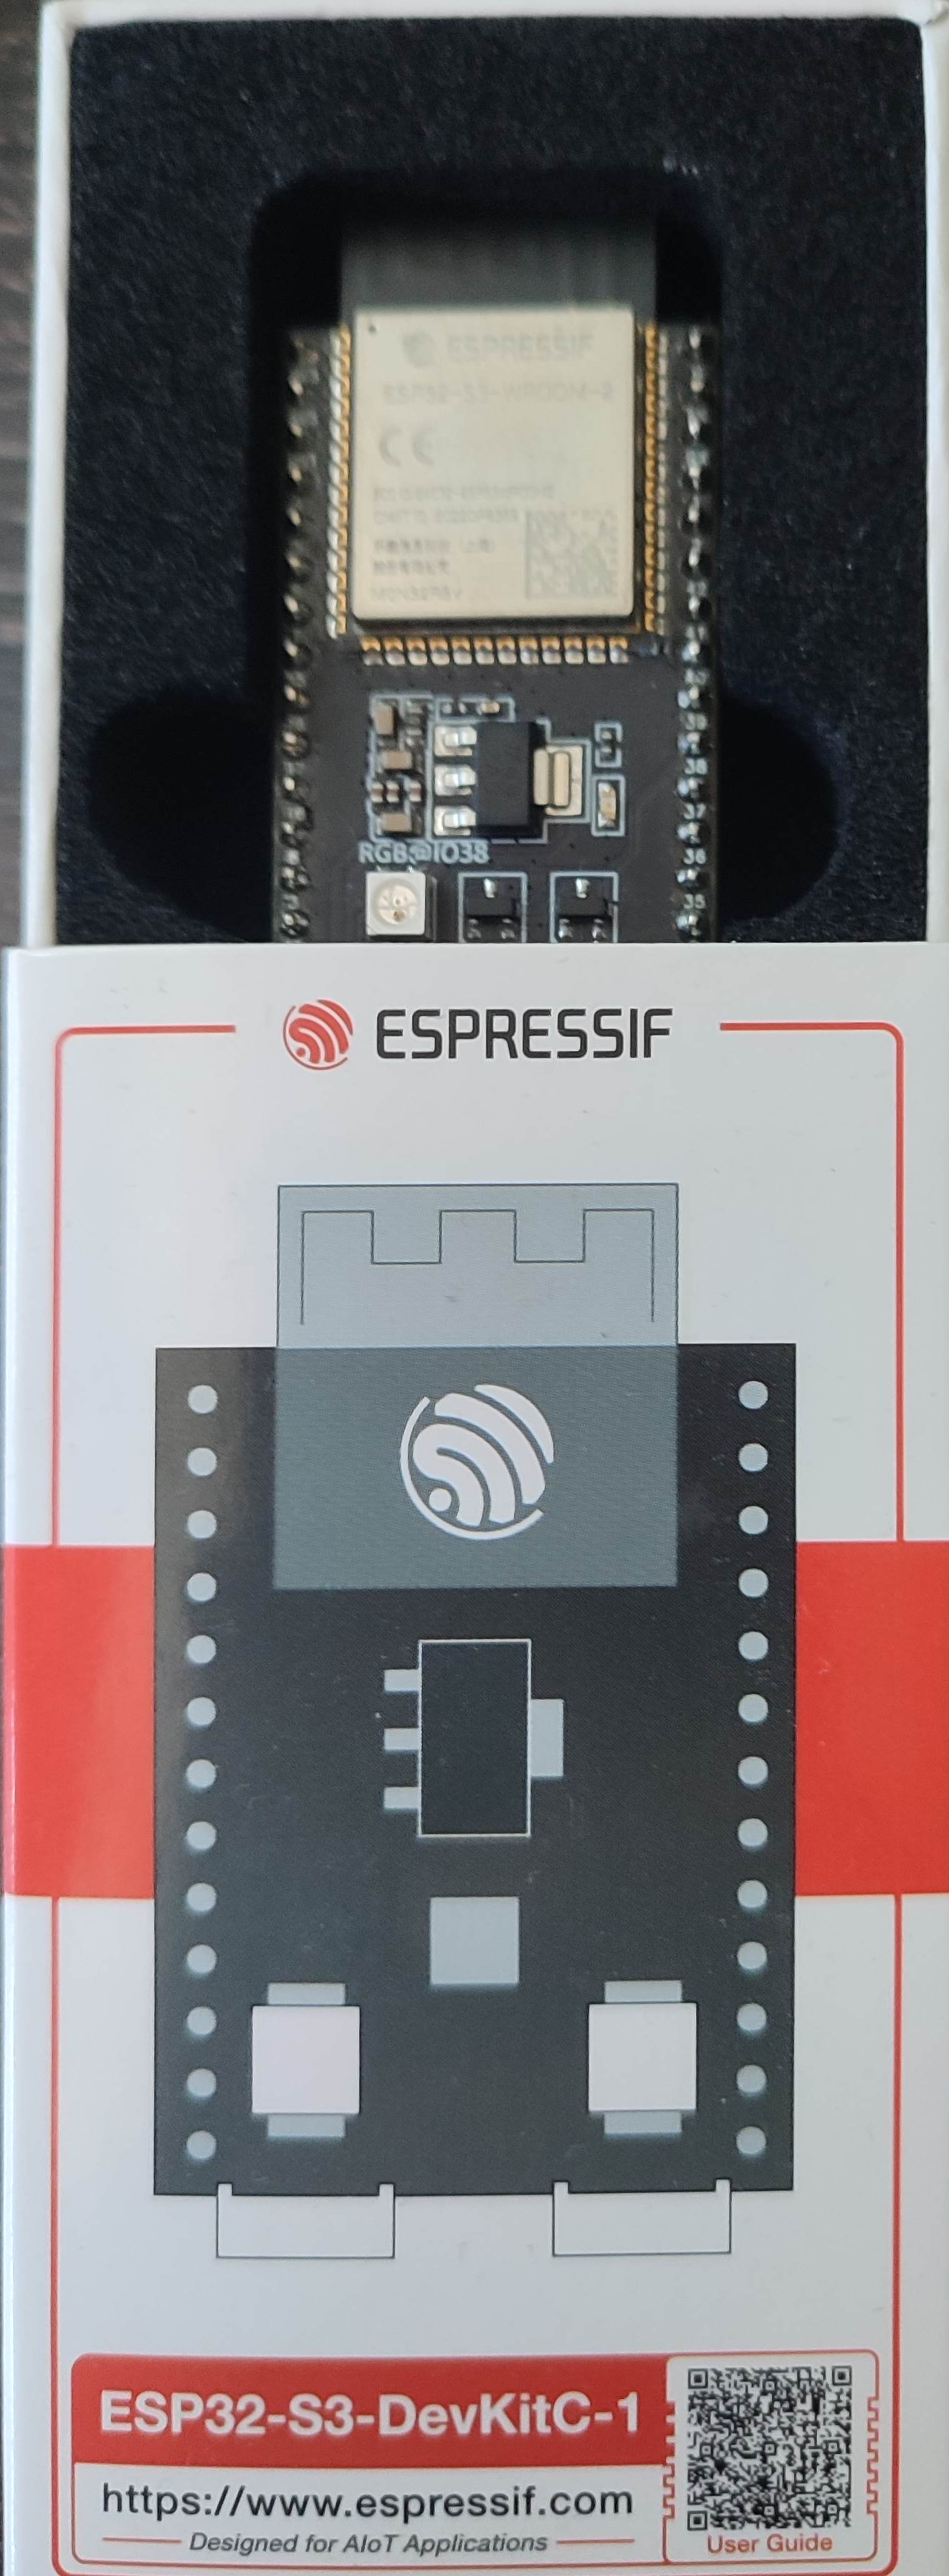
\includegraphics[width=3cm]{MyESP32}
		\caption{Általam használt ESP32 modell}
		\label{img_myesp}
	\end{figure}
	
	Ezen eszközök számos bemeneti és kimeneti perifériákkal rendelkeznek:
	\begin{itemize}
		\item Digitális I/O pin-ek
		\item Analóg bemenetek (ADC\footnote{Analog to Digital Converter, lehetővé teszi az áramkörben érzékelt analóg jelek feldolgozását.})
		\item Digitális-analóg átalakítók (DAC\footnote{Digital to Analog Converter, lehetővé teszi az áramkörre kibocsájtott feszültség modulálását.})
		\item PWM (Pulse Width Modulation\footnote{Ezen technológia teszi lehetővé a DAC működését.}) kimenetek
		\item SPI, I2C, UART kommunikációs interfészek
	\end{itemize}
	Ezek a csatlakozók lehetővé teszik különböző érzékelők, kijelzők és egyéb perifériák csatlakoztatását.
	Ezeket az eszközöket nagyrészt C és C++ nyelven lehet programozni, azonban van lehetőség a MicroPython és Lua script nyelvek használatára.
	\section{A rendszer fejlesztésének részletei}
	A fejlesztés folyamatát szokásos módon két részre bonthatjuk, elsősorban a hardver fejlesztésére, majd a szoftver fejlesztésére.
	\subsection{Hardver szintű fejlesztés}
	A projekt megvalósításához szükség volt egy egyedi áramkörre, amivel maximalizálhatom az elérhető portok számát.
	\begin{figure}[!ht]
		\centering
		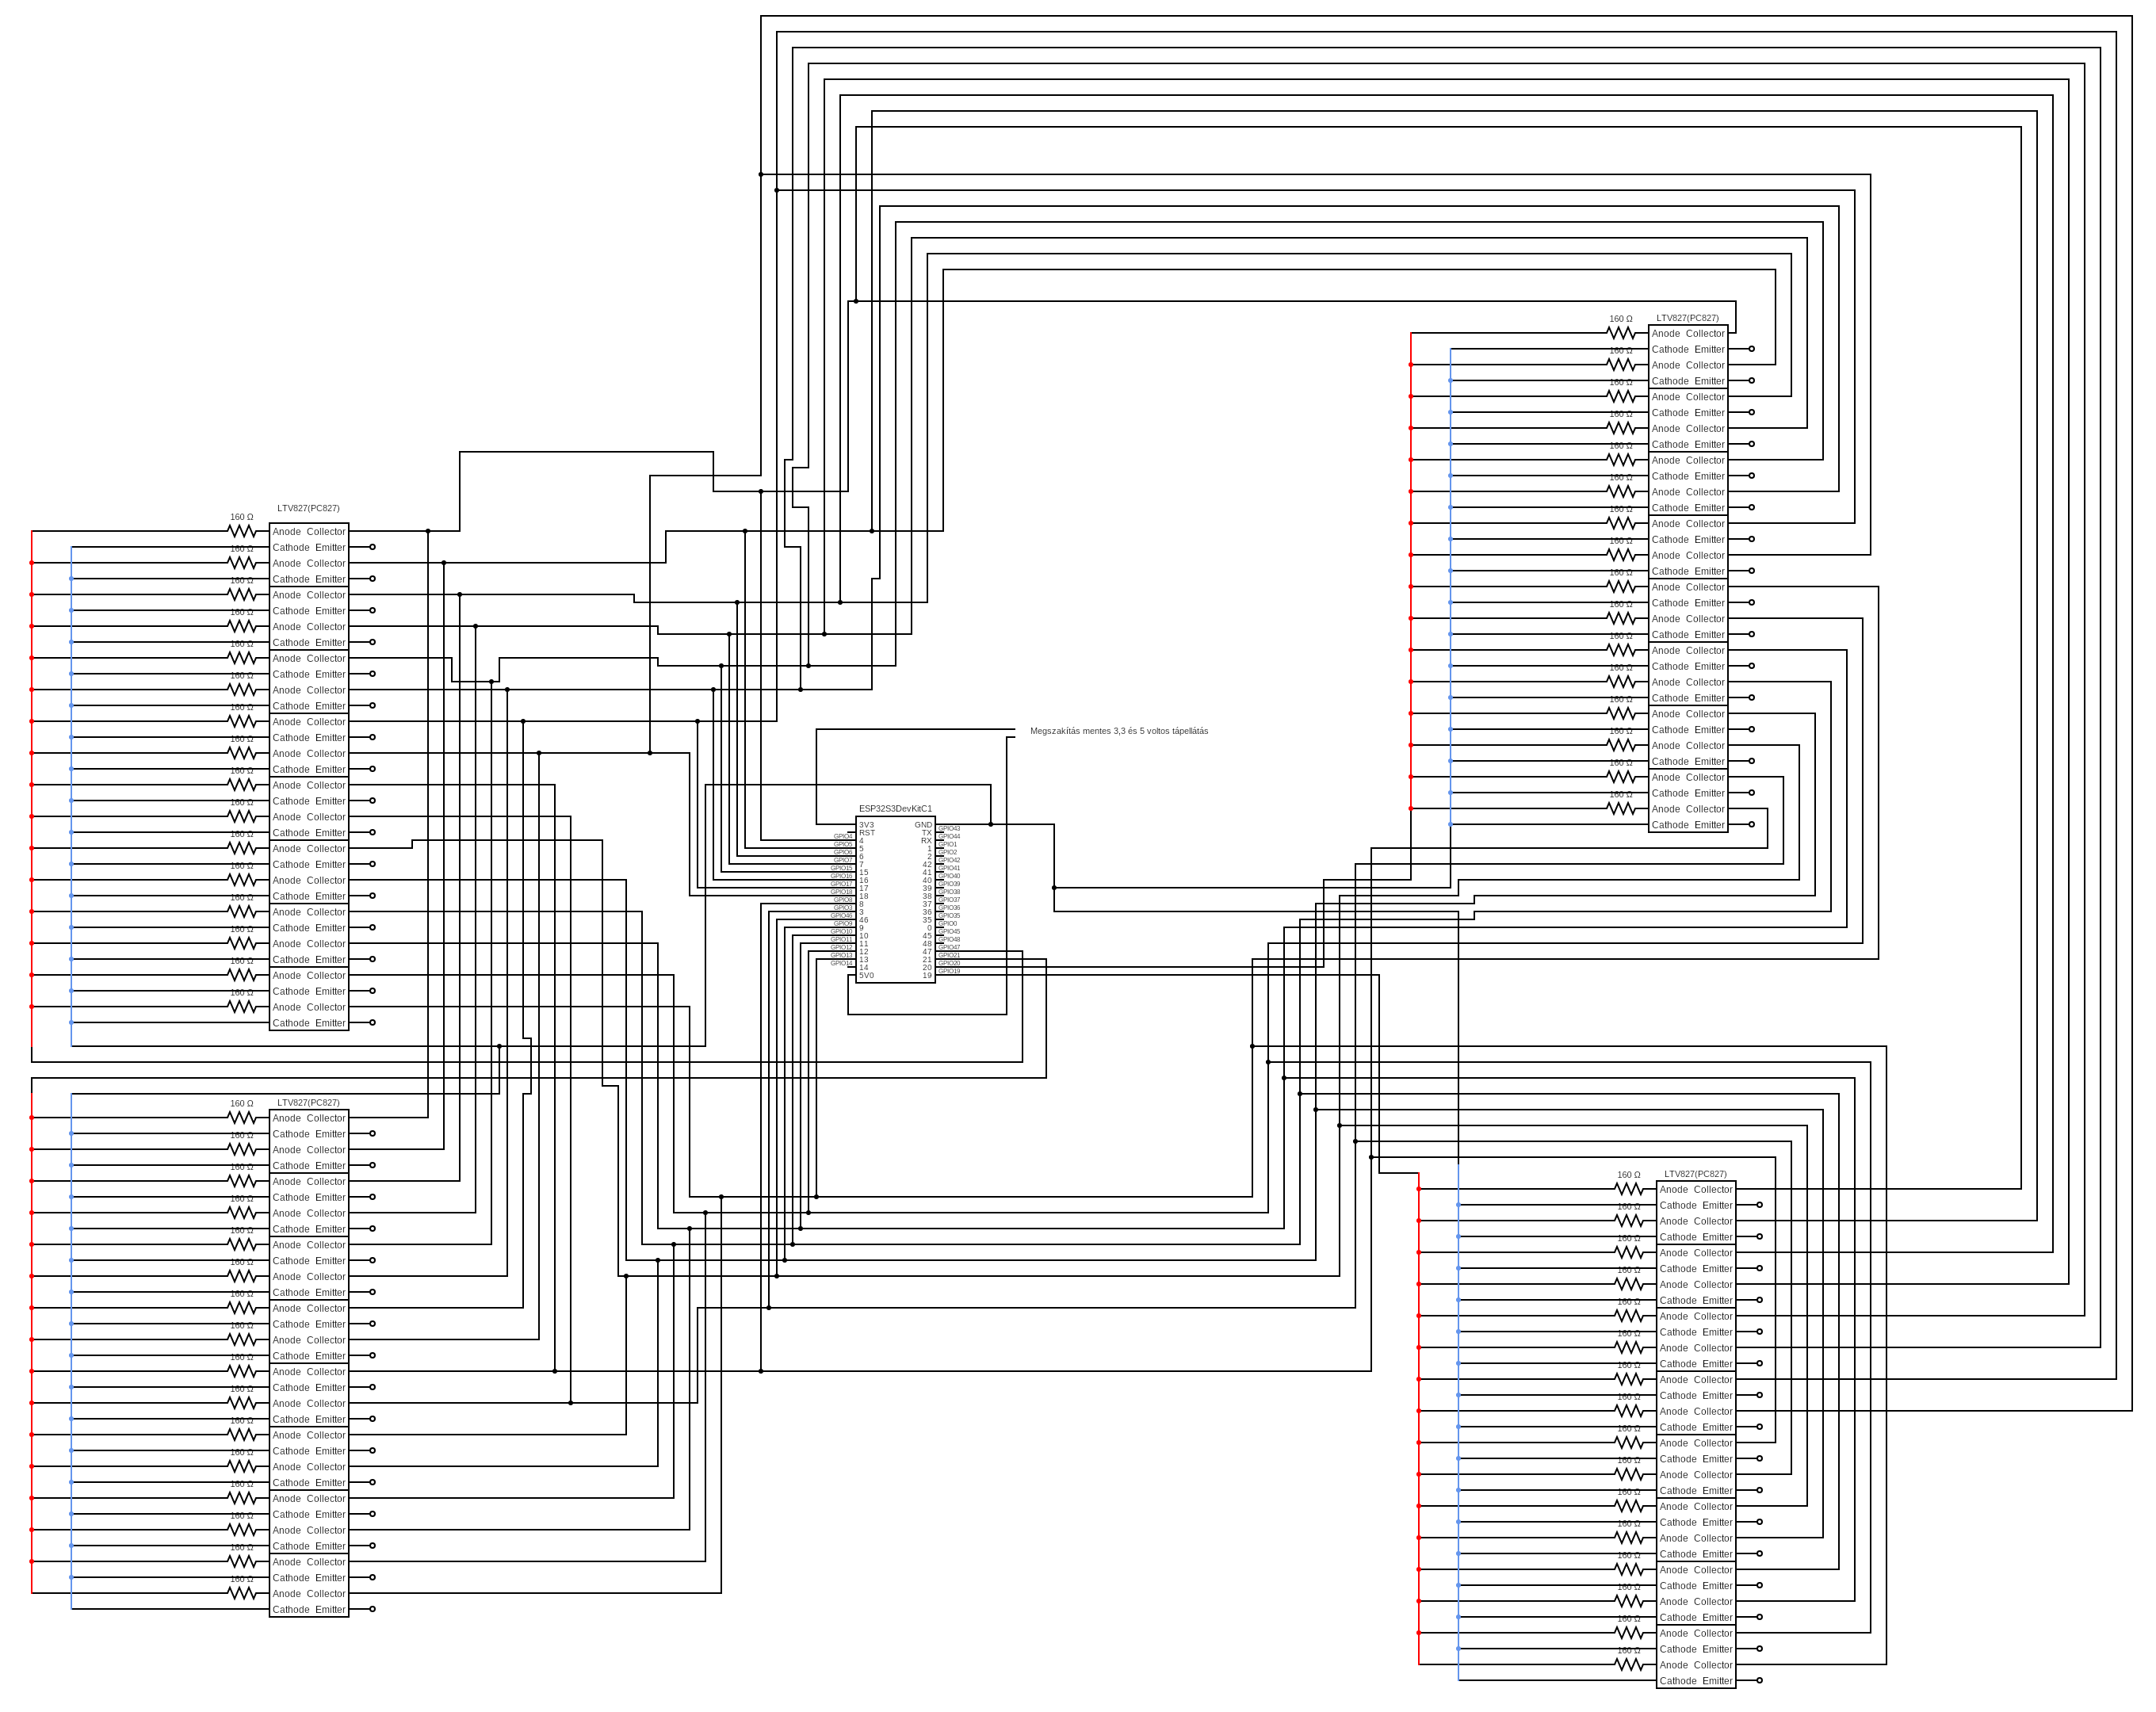
\includegraphics[width=10cm]{circuit}
		\caption{Hatékonyság növelés érdekében kifejlesztett egyedi áramkör.}
		\label{img_circ}
	\end{figure}
	A \ref{img_circ}-es ábrán látható az említett áramkör, amely segítségével elérem az általam elfogadható eredményt. Ebben a kulcsfontosságú alkatrészek az optocsatoló, amelyek használatával igyekeztem  az esetlegesen előforduló interferenciát csökkenteni.
	Ez a kapcsolási rajz a \href{https://www.circuit-diagram.org/}{\color{blue}{Circuit Diagram}} segítségével készült.
	Az ábra nem tartalmazza az érzékelő vezetékeket, amivel az eszköz érzékeli, hogy csatlakoztatva van-e a modul.
	
	A kapcsolási rajz nem nevezhető egyértelmű bizonyítéknak annak helyességéről. Így prototípus készítése ajánlott. Egy ilyen prototípus tekinthető meg a \ref{img_proto}.~képen.
	\begin{figure}[!ht]
		\centering
		\includegraphics[height=10cm]{korai_prototipus}
		\caption{Kapcsolási rajz alapján készült prototípus, egyéb teszteléshez használt komponensekkel.}
		\label{img_proto}
	\end{figure}
	\subsection{Szoftver fejlesztése és a fejlesztés során felmerült problémák}
	\label{sub_fejlESP}
	Fejlesztés elején több probléma is felmerült.
	\begin{enumerate}
		\item A modul vezérlő fájlok tárolása. Amennyiben C++ vagy C nyelvet használunk a belső tárhely kizárólagosan az általunk feltöltött fájlokat tartalmazza és a hozzáférés nehézkes fájlrendszer nélkül. Szerencsére elérhető több csomag is ennek a megoldására, mint a \href{https://github.com/littlefs-project/littlefs}{\color{blue}{LittleFS}}, vagy a \href{https://docs.espressif.com/projects/esp-idf/en/stable/esp32/api-reference/storage/spiffs.html}{\color{blue}{Spiffs}}
		\item A modul vezérlő fájlok használata, vagy futtatása. A projekt egyik fő feladata, hogy a modulok programja és a fő program egymástól függetlenül legyenek képesek működni, azaz ne a fő program hajtsa végre a szükséges lépéseket, hanem a modul vezérlő. Egy megoldás erre a fájl dinamikus betöltése és a program belépési pontjának meghatározása, majd a pont memória címén keresztüli futtatás. Ez a megközelítés a programot rendkívül bonyolultá tette volna és memória biztonsági problémákat is felvetett volna, mivel a C++ nyelvben íródó programnak C-t is használnia kellett volna.
	\end{enumerate}
	 Ez a kettő komolyabb probléma vezetett arra, hogy más nyelvet keressek. A MicroPython mind a kettő problémára megoldást nyújtott a beépített fájlrendszerével és JIT\footnote{Just In Time} interpreterével, ugyanis így nem bináris kóddal kell dolgozni, hanem egyszerű \textit{.py} fájlokkal.
	 Ez a változtatás nagyban megkönnyítette a program fejlesztését.
	 
	 A váltás után neki tudtam kezdeni a tényleges fejlesztésnek. Itt a főbb problémákat a fájl letöltése és azoknak a futtatása jelentette. A fájl letöltését több módszerrel is megkíséreltem, azonban egyik sem hozott megfelelő eredményt, végül a Google API használatával sikeresen le tudtam tölteni a fájlt. Az API mindössze a Google-től igényelt API kulcsot és a fájl azonosítóját kéri (Az azonosító a megosztási linkből kinyerhető.).
	 
	 Ezen a ponton a szerverrel való kommunikáció is kérdéses volt. Elsőre Websocket technológiát terveztem használni, azonban ezt drágának találtam és a szervernek egyszerre több kapcsolatot is fenn kellett volna tartania, miközben relatívan kevés és ritka az információ áramlása. A következő ötlet egy az eszközön futó API volt, ez azonban ennek a megoldásnak, hogy működőképes legyen szükséges az eszköz IP címe, valamint esetlegesen portforwarding-re van szükség amely nem egyezik az eszköz Plug\&Play irányzatával. Ennek eredményéül a jól ismert RestAPI technológia mellett döntöttem. Az API-ról többet olvashat a \ref{ch_API}.~fejezetben.
	 
	 API-ra még így szükség van a konfigurációhoz, ehhez a Microdot könyvtárat használtam, valamint a szerver felé irányuló kérésekhez a urequests és az abból származó adatok feldolgozásához a nyelv által alapértelmezetten tartalmazott modulokat használtam, például a \textit{ujson} modult. A konfigurációhoz használható más technológia az eszköz esetében a Bluetooth volt, azonban ezt az egyszerűség kedvéért nem használtam.
	 
	 \begin{megjegyzes}
	 	A Bluetooth-os konfiguráció kihagyása, jó döntés volt. A Tarlogic Március 6.~megjelent cikk-je alapján\cite{bib_esp_bluetooth}. A cikk említést tesz egy több millió eszközt sújtó sebezhetőségi pontról. A cikk által említett eszközök Bluetooth chipjeiben rejtett funkcionalitást véltek felfedezni, amely biztonsági résként fogható fel.
	 \end{megjegyzes}
	 
	 A felhasználónak mindenféle képen jelezni kell az eszköz belső állapotáról, ennek a legegyszerűbb formája a színek használata, szerencsére az eszköz el van látva egy  beépített NeoPixel LED-el, amely használatához a NeoPixel könyvtárra volt szükségem.
	 
	 A konfigurációhoz és működéshez szükséges a MicroPython-ban alapértelmezetten megtalálható network modul. A modul segítségével tud az eszköz létrehozni saját WiFi hálózatot, valamit csatlakozni egy már meglévő hálózathoz. Szintén alapértelmezett csomag az OS csomag, amely a legtöbb Python verzióban megtalálható. Ez a könyvtár rendkívül fontos az eszköz működésének szempontjából, mivel használatával dönthető el, hogy bizonyos fájlok, például az eszköz saját azonosítóját tartalmazó fájl jelen van-e a fájlrendszerben.
	 
	 A műveletek megvalósítása egy végtelen ciklusban történik, ahol minden iteráció egy a szerver felé irányuló kéréssel kezdődik. A végpont amely kezeli ezt a kérést az egyetemen tanultaktól eltér, a végpontról többet olvashat a \ref{ssec_long_polling}.~szekcióban. Innentől az esetlegesen több feladatot egy a végtelen ciklusba beágyazott \textbf{for} ciklus kezeli, amely törzsében minden egyes feladatot megvizsgálunk.
	 
	 A ciklus törzsében található if-elif szerkezet döntéshozó szervként működik. A feladat, mint JSON dokumentum \textit{aditionalInfo} mezőjében található \textit{method} mező rejti a feladat típusát, ezek a típusok és hozzájuk társított folyamatok megtekinthetőek a \ref{sec_mukodes}.~szekcióban található felsorolásban.
	 
	 Ezen folyamatok közül a legnehezebben a ,,run'' volt megvalósítható. Itt a modulhoz társított python fájl azonosítója alapján választjuk ki a tárolt modulok közül a feladatban megadott modult. Minden modulhoz tartozik egy metódus, például a az első számú modulhoz a ,,runa'' metódus tartozik. Ezek a metódusok kivétel nélkül el vannak látva egy dekorátorral, amely feladata a megfelelő áramkör kiválasztása. Ezen metódusok belsejében hívódnak meg a különböző modulok ,,run"" metódusai, amely egy paraméterrel van ellátva. Ez a paraméter tartalmazza a feladat paramétereit.
	 
	 
	 
	 \section{Az eszköz működése}
	 \label{sec_mukodes}
	 Az eszköz használata konfigurációval kezdődik, melyet kék fénnyel jelez a felhasználónak. A konfiguráció után megpróbál csatlakozni a megadott hálózathoz eközben az eszközön található LED kék fényről pulzáló zöld fényre vált. Amennyiben a kapcsolódás sikeres az eszköz zöld fénnyel jelzi ezt, ha sikertelen, akkor újraindul a folyamat.
	 
	 Sikeres kapcsolódás után önmagát regisztrálja az eszköz a hálózatra. Innentől az eszköz használatra kész és azonnal kérést küld az API-nak a hozzá kapcsolt feladatok iránt érdeklődve. A szerver válasza alapján a következő műveleteket végezheti el az eszköz:
	 \begin{itemize}
	 	
	 	\item ,,add\_new'': A parancs kiadásával új modult tudunk hozzáadni az eszközhöz.
	 	\item ,,remove'': Az ,,add\_new'' parancs ellentettje. Modul eltávolítására adja ki a parancsot.
	 	\item ,,disown'': Gyári visszaállítás.
	 	\item ,,network\_reset'': Az eszköz elfelejti a hálózatot. Hasznos lehet, ha az eszközt egy másik épületbe helyezzük át.
	 	\item ,,module\_reset'': Az eszköz belső állapotát visszaállítja, ezzel egyszerre az összes modul eltávolítható.
	 	\item ,,run'': Futtatja a modulhoz megadott programot.
	 \end{itemize}
	 Fontos megjegyezni, hogy minden feladat elvégzése annak törlésével és egy új kéréssel záródik. A ,,run'' parancs esetén az eszköz a modul azonosítója alapján dönti el, hogy melyik modult kell használnia, azaz megállapítja a modul áramkörét és kiválasztja azt. Az ,,add\_new'' esetén az eszköz újraindul, hogy a program sikeresen érzékelni tudja a fájl változásait, erre a ,,remove'' parancs esetén nincs szükség, mivel a program belső állapota változik csak.
	 
	  Az eszköz esetleges áramkimaradásra fel van készítve, mivel a belső állapot változása folyamatosan mentve van a belső tárhelybe.
	\chapter{A REST API fejlesztése}
	\label{ch_API}
	Az API az Express.js keretrendszerrel készült és minden entitás CRUD műveleteit ellátja.
	\section{Adatbázis kezelése}
	Az adatbázishoz egy egyszerű connect stringel történik, amelyet a MongoDB oldalán kérhetünk. A string tartalmazza a felhasználónevet, fiókhoz tartozó jelszót és más az adatbázissal kapcsolatos adatokat, mint az appName paramétert.
	
	A kapcsolat létesítéséhez szükség van a MongoDB natív JavaScript driver-ére, ezt az NPM segítségével letölthetjük, majd az ebben található MongoClient osztályt importálhatjuk és új példányt hozhatunk létre, az osztály konstruktora a már feljebb említett connect stringet várja paraméterül. Innentől kiválaszthatjuk az adatbázist amin dolgozni fogunk.
	
	A programkódban minden collection-re külön fájl készült.  Az adatbázishoz tartozó metódusok mindig egy JSON objektumot várnak. A műveletek elvégzését MongoBD által definiált metódusok hívásával lehetségesek. Az adatbázis különbséget tesz az alapján, hogy egy vagy több dokumentumot várunk eredményül, ez az összes metódusra igaz. A collection-ben való keresés nem nehéz, csak meg kell adni a mező nevét és annak értékét, ez azonban nem annyira egyszerű, ha a ,,\_id'' mező alapján akarunk keresni, hiszen az eddigiek alapján arra készülünk, hogy a megfelelő mezőhöz kell kapcsolni az adatot, azonban ahogy a \ref{lst_docu}.-es dokumentumban láthatjuk a mező nem string hanem objektum típusú, ez azonban nem észrevehető, ha a klienst, vagy a weblapot használjuk. A dokumentációt\cite{bib_mongo_docs} keresve nem találtam megoldást így a fórumhoz\cite{bib_mongo_forum} fordultam, ahol megtaláltam amit kerestem. Ahhoz, hogy ID alapján tudjunk keresni szükségünk van az ,,ObjetId'' nevű osztályra, ennek a konstruktorába kell elhelyezni az ID-t.
	
	\section{Végpontok}
	Ahogy az adatbázis kezelésnél itt is minden collection-nek külön fájl van dedikálva, nagy részük nem különbözik a már megszokott végpontoktól. Azonban, az nem optimális, ha az okos eszköz folyamatosan kéréseket küld az API-nak. A probléma megoldása az IoC\footnote{Inversion of Controll} alkalmazása, akár csak a modern GUI-val ellátott alkalmazások esetén. Nem a program vár vezérlésre, hanem majd jelzünk a programnak, hogy végezze el a feladatot. Ez azt jelenti, hogy az API-nak kell jeleznie az okos eszköznek a feladat elvégzésére. Erre egy jó megoldás lehet az RPC\footnote{Remote Procedure Call}, azonban így a szervernek tudnia kell az eszköz IP címét, valamint portforward-ot kell végeznünk.
	\subsection{Mi felel meg az elvárásoknak?}
	Elvárásaink:
	\begin{enumerate}
		\item Az eszköznek kell kezdeményezni a kapcsolatot, ezzel elkerülve a lehetséges problémákat melyeket a hálózat, vagy a tűzfal okozhat. \label{it_elv_1}
		\item Az eszköznek várnia kell a feladatra, nem küldhet request-et percenként a szervernek. \label{it_elv_2}
		\item Az eszközt értesíteni kell a feladat létrejöttéről, akárcsak az Observer.\label{it_elv_3}
	\end{enumerate}
	Ezen elvárásoknak megfelel például a WebSocket, azonban ezt túlságosan pazarló megoldásnak találtam, ahogy a \ref{sub_fejlESP}.-es szekcióban is említettem. Egy másik Lehetőség az SSE\footnote{Server Sent Event}-volt, azonban míg könnyű implementálni a kapcsolat csak egy irányú, ezáltal az eszköz nem küldhet vissza adatot a szervernek\cite{bib_SSE}. Az SSE-ről többet olvashat a \ref{sssec_SSE}.~szekcióban, valamint megtekintheti az SSE és WebSocket összehasonlítását a \ref{tab_sse_v_websocket}.~táblázatban.
	
	Egy másik lehetőség az MQTT\footnote{Message Queuing Telemetry Transport} volt, amely IoT felhasználásra tökéletes, azonban, hogy ez működjön szükségünk van egy broker-re pl.: Mosquitto, AWS IoT. Ez egy plusz költséget jelent a rendszerben, amely drágábbá tenné a rendszert, ez nem lehetőség\cite{bib_MQTT}. Az MQTT-ről többet olvashat a \ref{sssec_MQQTT}.~szekcióban.
	
	Egy pénzügyileg kedvezőbb megoldás a Polling. Amely HTTP protokollal tökéletesen működik és eleget tesz az \ref{it_elv_1}.~feltételnek és a \ref{it_elv_3}.~kritériumnak is, azonban ebben az esetben az eszköz bizonyos intervallumonként újra kérést fog küldeni a szervernek, ez a \ref{it_elv_2}. pontnak nem felel meg.
	
	A Polling egy változata a Long-Polling azonban megfelel az elvárásainknak. A módszer implementálásával, az eszköz addig várakozik a válaszra amíg azt meg nem kapja, majd annak érkezésével végrehajtja az abban kapott feladatot és az esetleges eredményeket vissza is tudja küldeni. 
	\subsubsection{Megfontolt technológia, SSE}
	\label{sssec_SSE}
	Az SSE (Server-Sent Events) egy olyan HTTP-alapú technológia, amely lehetővé teszi, hogy a szerver valós időben küldjön adatokat a kliensnek egy egyirányú kommunikációs csatornán keresztül. Az SSE-t gyakran használják valós idejű értesítések, frissítések és adatstreamelés céljaira, ahol a kliensnek folyamatosan frissülő információra van szüksége anélkül, hogy újra és újra lekérdezné a szervert\cite{bib_SSE_spec,bib_SSE}.\\
	\textbf{Működési elv}\\
	Az SSE a standard HTTP/1.1 vagy HTTP/2 protokollt használja, és egy tartós TCP-kapcsolaton keresztül működik. A kliens (általában egy böngésző) létrehoz egy kapcsolatot a szerverrel egy speciális EventSource API segítségével, majd a szerver folyamatosan küldhet eseményeket a kliens felé text/event-stream MIME típusban.\\
	\textbf{SSE jellemzöi}\\
	\begin{enumerate}
		\item Egyirányú kommunikáció –- Csak a szerver küldhet adatot a kliens felé.
		\item Egyszerű implementáció –- Nincs szükség komplex protokollokra (mint a WebSocket).
		\item HTTP-alapú –- Nem igényel külön portot, működik a meglévő HTTP(S) infrastruktúrán.
		\item Automatikus újrakapcsolódás –- Ha a kapcsolat megszakad, a kliens automatikusan újrapróbálkozik.
		\item Támogatja az eseménytípusokat -– Lehetőség van különböző típusú események küldésére (pl. message, update).
	\end{enumerate}
	
	\begin{table}[!h]
		\centering
		\caption{SSE és WebSocket összehasonlítás}
		\label{tab_sse_v_websocket}
		\begin{tabular}{|l|l|p{5cm}|}
			\hline
			\textbf{Jellemző}         & \textbf{SSE}                          & \textbf{WebSocket}                  \\ \hline
			\textbf{Kommunikáció iránya}       & Egyirányú (szerver $\rightarrow$ kliens) & Kétirányú (duplex)                  \\ \hline
			\textbf{Protokoll}                 & HTTP/HTTPS                            & WS (WebSocket), WSS (secure)        \\ \hline
			\textbf{Adatformátum}              & Csak szöveg (text/event-stream)       & Szöveg és bináris is                \\ \hline
			\textbf{Komplexitás}               & Egyszerű (beépített böngésző API)     & Bonyolultabb (külön könyvtár kell)  \\ \hline
			\textbf{Újrakapcsolódás}           & Automatikus                           & Manuális kezelés szükséges          \\ \hline
			\textbf{Alkalmazási terület}       & Valós idejű értesítések, frissítések  & Chat, játékok, valós idejű interakció \\ \hline
			\textbf{Böngészőtámogatás}        & Modern böngészők (IE nem)            & Szélesebb támogatás                 \\ \hline
		\end{tabular}
	\end{table}
	\FloatBarrier
	\subsubsection{MQTT, mint megfontolt protokoll}
	\label{sssec_MQQTT}
	Az MQTT egy nyílt, könnyűsúlyú üzenetküldő protokoll, amelyet eredetileg a publisker-előfizet (pub/sub) modellre terveztek az alacsony sávszélességű, magas késleltetésű hálózatok (pl. IoT eszközök) számára. Az MQTT-t ma széles körben használják az Ipari Internet of Things (IIoT), otthoni automatizálás, és valós idejű adatátviteli rendszerek területén. A protokollt az OASIS szabványosította, és a ISO/IEC 20922 szabvány részét képezi\cite{bib_MQTT_iso,bib_MQTT_oasis}.\\
	\textbf{Történet és fejlődés}
	\begin{itemize}
		\item 1999: Az IBM és az Arcom (ma Eurotech) fejlesztette ki Andy Stanford-Clark és Arlen Nipper vezetésével, olajvezeték-figyelő rendszerekhez\cite{bib_MQTT_ibm}.
		\item 2014: Az MQTT v3.1.1 vált hivatalos OASIS szabvánnyá.
		\item 2019: Megjelent az MQTT v5, új funkciókkal (pl. üzenetlejárat, okokódok, megosztott előfizetések).
	\end{itemize}
	\textbf{Működési elv (Publish-Subscribe modell)}\\
	Az MQTT központi broker segítségével működik, amely üzeneteket továbbít a kliensek között. A kommunikáció témakörök (topics) alapján történik.
	Kulcsfogalmak:
	\begin{enumerate}
		\item Közzétevő (Publisher): Üzeneteket küld egy témakörre (\textit{publish}).
		\item Előfizető (Subscriber): Feliratkozik egy témakörre, és fogadja az üzeneteket (\textit{subscribe}).
		\item Broker: Közvetíti az üzeneteket a megfelelő előfizetőknek.
		\item Témakör (Topic): Hierarchikus útvonal (pl. \textit{iot/sensor1/temperature}).
	\end{enumerate}
	\subsection{Long-Polling megvalósítása}
	\label{ssec_long_polling}
	Tekintve, hogy Long-Polling-ot még nem használtam meg kellett ismernem\cite{bib_long_poll1,bib_long_poll_imp}. Ezek mellett praktikusabb példákat is keresnem kellet, hogy jobban megértsem\cite{bib_long_poll_pl}.
	
	Implementálás után teszteltem a funkciót, eleinte jól működött, azonban amikor több feladatot is feltöltöttem az API összeomlott és az eszköz kommunikációs hibát dobott. A hiba gyökere az volt, hogy, míg a bejövő request elindította a folyamatot, addig egy másik ismét megtette ezt, így a kapcsolat a response elküldésével lezárult és nem tudta az API elküldeni a másikat. Ennek megoldása ként egy ,,jelenleg futó'' másodlagos lista létrehozása volt szükséges.
	\lstinputlisting[style=JavaScript,label=lst_polling_p1,caption={Long-Polling-hoz tartozó végpontok és tömbök.}]{sample_of_long-polling_p1.js}
	A kommunikáció hatékony, IoC szerű működésének megvalósításához szükséges végpontok a \ref{lst_polling_p1}.~kódrészleten láthatóak, amelyek feladata az
	\begin{itemize}
		\item eszköztől érkező kérések fogadása és megtartása, abban az estben, amikor nem érhető el adat, (Ez a feladat a ,,GET'' végpontra hárul. A végponton belül még szükséges több ellenőrzést elvégezni a megfelelő működés érdekében.)
		\item a ,,POST'' végpont használatakor egy keresés indul el, amely lehetővé teszi az eszköz kérésére a válasz mihamarabbi megadását, amennyiben a cél eszközhöz társul adat a responses tömbön belül. (Ezzel a megoldással elkerülhető a folyamatos, ciklikus megfigyelés, amely rendkívül költséges lenne.)
	\end{itemize}
	A két végpont közt kialakuló rendszerszerűség felfogható egyfajta megfigyelő (Observer) tervezési minta használataként.
	\lstinputlisting[style=JavaScript,label=lst_polling_p2,caption={Long-Polling működéséhez szükséges metódusok.}]{sample_of_long-polling_p2.js}
	A \ref{lst_polling_p2}.~kódrészletben található metódusok elősegítik a \ref{lst_polling_p1}.~kódrészletben látható végpontok által megvalósító Long-Polling mechanizmus működését. Tekintettel a metódusok számára a legegyszerűbb áttekintést egy felsorolás adja.
	\begin{itemize}
		\item \textbf{checkForData}: A metódus célja egyszerű. Visszaadja az eszközre vonatkozó elem indexét.
		\item \textbf{getExec}: Célja rendkívül hasonlít a \textit{checkForData}-ra, azonban a jelenleg végrehajtás alatt lévő válaszok listájában keres.
		\item \textbf{remove}: A Long-Polling által használt két tömbből távolítja el az adatokat, ezzel elkerülve, a feladatok nem kívánt ismétlését és esetleges bejövő feladatok blokkolását.
		\item \textbf{executeByIndex}: A metódusara a Long-Polling igáslovaként tekinthetünk. Feladata a többi metódus használatával a feladat előállítása és továbbítása az eszköz felé.
	\end{itemize}
	
	\chapter{Frontend program fejlesztése}
	Tekintettel a Flutter fejlesztéssel kapcsolatos hiányosságomra, a fejlesztés az alapvető fogalmak és tudás elsajátításával kezdődött. Nem csak a Flutter-t mint keretrendszert, hanem a Dart nyelvet is meg kellett ismernem. Ez különböző ,,crash course'' videók segítségével  történt\cite{bib_flutter_fireship,bib_flutter_traversy,bib_flutter_freecodecamp}. Ezen hiányosságok miatt ez a fejezet hosszabb a többinél, ugyanis a technológiával kapcsolatban számos új tapasztalatot szereztem.  A fejlesztés alatt továbbá ihlet szerzéséhez használtam némelyik forráshoz tartozó repozitóriumokat is \cite{bib_flutter_freecodecamp_repo,bib_flutter_traversy_repo}.
	\section{UI fejlesztés Flutter keretrendszerben}
	Ezen szekció a felhasználó felület fejlesztése közben szerzett tapasztalatot hívatott összefoglalni.
	\subsection{Grafikus felhasználói felület fejlesztése Flutter-ben}
	A Flutter esetében minden UI elem egy Widget ősosztályból származik. A Widgetek kivétel nélkül tartalmaznak egy példányt a  ,,BuildContext'' osztályból, amelyre tapasztalat szerint mindig ,,context'' névvel hivatkozunk.
	
	Amennyiben teljesen új felületet hozunk létre szükségünk lesz kettő osztályra. Az első osztályt, vagy a ,,StatelesWidget'', vagy a ,,StatefulWidget'' osztályból származtatjuk, majd a másik osztályunkat egy ,,State'' generikusból származtatjuk, olyan módon, hogy az első osztályunk lesz a típusa. Erreláthatunk példát a \ref{lst_page_creation}.~kódrészletben.
	\lstinputlisting[language=Dart,label=lst_page_creation,caption={Felülettel kapcsolatos osztályok és azok kapcsolata.}]{page_creation.dart}
	A már említett kódrészleten észrevehető a ,,\_'' karakter. Ennek használatáról többet olvashat a (itt lesz egy dart részlet).~szekcióban, amelyben a Dart nyelvet tárgyaljuk felületesen.
	
	Az osztályokban általában egy-egy metódust írunk felül. A ,,Test'' osztályban a ,,createState'' és a ''\_TestState''-ben a ,,build'' metódust. Felhasználói felület kialakításánál a build metódusra koncentrálunk, ugyanis ez ad vissza Widget típust.
	
	Általánosságban a ,,Scaffold'' Widget használatával kezdünk, amelyben a felületet a body paraméter megadásával kezdjük, amely több egy Widget típusú osztályt fog tartalmazni. Ez bármelyik osztály lehet. Vannak osztályok amelyek egy, vagy, akár  több osztályt képesek befogadni. A Scaffold-nak a body-n kívül még van egy ,,appBar'' paramétere, ez a paraméter egy AppBar osztályt fogad, amelyben cím, háttérszín, egyéb paraméterek és egy ,,actions'' paraméter adható meg. A többesszámból könnyen felismerhető, hogy ez a paraméter több Widget-et is képes fogadni, ezek például lehetnek különböző gombok.
	\subsection{Navigáció a felületek között}
	A Flutter a navigációt egy veremmel oldja meg. Ez által amikor át akarunk lépni egy másik lapra, kivétel nélkül a ,,Navigator'' osztály használatos. Ez által a vermek szokásos metódusai használhatóak a navigációhoz, kisebb módosítással és bővítéssel. Tekintsük azt az esetet amikor nem akarjuk a felhasználót vissza engedni az előző lapra, ebben az esetben a ,,pushReplacement'' metódus használatos.
	
	A BuildContext-et nem csak felület elemei használják, hanem a navigációhoz szanált osztály metódusai is. Tekintve a visszalépést az előző oldalra (vagy felületre), a vermeknél megismert pop metódust használjuk, Flutter-ben  ennek paramétere midig a kontextus (context). A BuildContext példányára nem csak visszalépés esetén van szükség, amennyiben egy másik felületre szeretnénk átirányítani a felhasználót, például egy gombnyomás esetén, a push metódust kell használnunk, amely egy két paramétert fogadó metódus. Az eddig leírtakból következtetve tudjuk, hogy a kontextusra lesz elsősorban szükségünk, a másik paraméter egy úgynevezett ,,MaterialPageRoute'' osztály, amely tartalmát a builder paraméterrel tudjuk megadni, ez általában a nyíl szintaxis\footnote{()=>} használatával történik.
	\subsection{A login page fejlesztése közben szerzett tapasztalatok}
	A fejlesztést a bejelentkező oldal készítésével kezdődött, ahol első sorban kialakításra került a grafikus interfész. Felismerve, hogy egyes elemeket a fejlesztés során többször használatba fogom venni, célszerűnek találtam egy gyűjtő osztály kialakítását, amely statikus metódusokat tartalmaz a különböző gyakran használt elemek legyártására, mint például a ,,TextField'' Widget. A különböző felhasználó által használt beviteli elemekből, mint a már említett ,,TextField''-ből az adatok kinyerése különböző módon történik, mint például egy WidowsForm programban. Flutter esetén szükségünk van egy ,,TextEditingController''-re, amelyt a mező létrehozásánál meg kell adnunk, ezen az osztályon keresztül tudjuk elérni a felhasználó által beírt adatokat.
	
	Az oldal kezdetleges tesztelése alkalmával, a jelszó mezőre kattintva megjelent egy ,,BottomOverflow'' üzenet, ahogy a \ref{img_login}.~képernyőképen látható. Ez az oldal kialakítása miatt történt. Magyarázata egyszerű: a megjelenő billentyűzet eltakarja a UI többi részét. Tekintve, hogy alapértelmezetten a ,,Column'' építőelem nem görgethető (scroll), a megoldást egy ,,SingleChildScrollView'' jelentette, amely gyermek attribútuma a már említett column lett.
	\begin{figure}[!h]
		\centering
		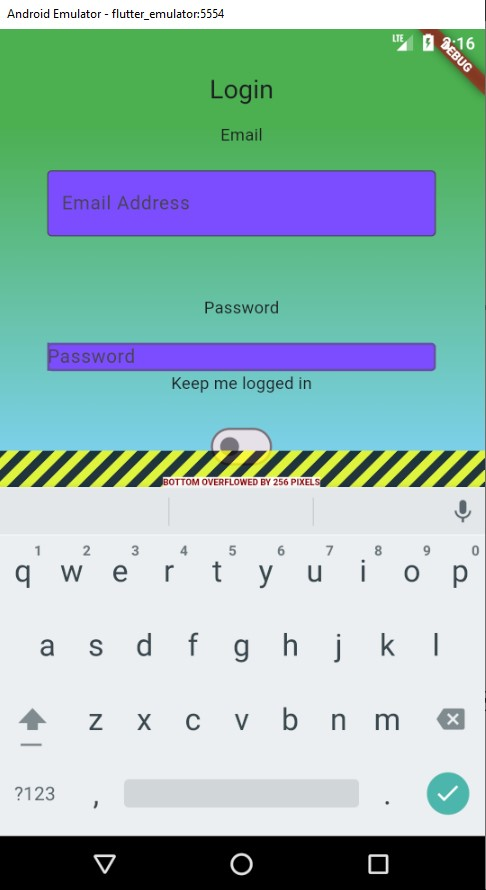
\includegraphics[height=10cm]{flutter_overflow}
		\caption{A képernyőre rálógó billentyűzet takarásáról szóló figyelmeztetés.}
		\label{img_login}
	\end{figure}
	
	Amennyiben a bejelentkezés sikeres volt, már csak egy dolgot kell tennünk. Ez az oldalak közötti navigáció.
	\subsection{Listák megjelenítése a Flutter keretrendszerben}
	Listák megjelenítése történhet statikusan és dinamikusan. Ebben a szekcióban dinamikus megjelenítést és felépítést tárgyaljuk.
	
	A dinamikus listák, avagy lista nézetek felépítésénél, szinte minden alkalommal a ,,ListView'' osztály egy külön konstruktorát használjuk. Ez lehet a ,,build'' konstruktor, vagy az általam használt ,,separated''. Ez a konstruktor legalább három paramétert vár.
	\begin{enumerate}
		\item ,,separatorBuilder'', amely a lista elemeit szétválasztó Widget-et gyártja le. Ez az én esetemben egy egyszerű Divider Widget volt.
		\item ,,itemCount'', ezen paraméter értéke útmutatóként szolgál a konstruktornak, hogy mennyi elem lesz a listView-ban.
		\item ,,itemBuilder'', feladata a lista elemeinek létrehozása. Minden esetben Widget típusú osztály egy példányát hozza létre, ez lehet egy egyszerű Container osztály, de akár az általam használt ListTile is.
	\end{enumerate}
	Fontos hogy minden dinamikusan felépített, valamint megjelenített ListView mögött egy lista áll, amely alapján létrehozható az.
	\subsection{Popup menük és dialógusok használata, megjelenítése}
	A popup menü használata jelentősen megkönnyítheti egyes felület elérését, vagy egy művelet elvégzését.
	A menü elkészítéséhez szükség van a ,,PopupMenuButton'' Widget-re, mely paraméterei a menü elemeinek megjelenítésére szánt ,,itemBuilder'' és az ,,onSelected'', amely a menü egyik elemének kiválasztásakor fog lefutni.
	A builder általánosságban egy ,,PopupMenuEntry'' típusú listát vár, amely tartalma a menü egyes elmei. Esetemben a listában ,,PopupMenuItem'' példányai találhatóak. Minden egyes elemnek tartalmaznia kell egy ,,value'' értéket, amely segítségével a már említett metódus felismerheti a kiválasztott elemet.
	
	A dialógusok használhatóak egyszerű értesítéshez, valamint megerősítés kéréséhez is. Elsőnek célszerű a dialógusok elkészítését áttekinteni.
	
	A dialógusok megjelenítéséhez a beépített ,,showDialog'' metódus használatos, amely paraméterei rendre a kontextus és a builder, amely felhasználja a kontextust. A builder tapasztalat szerint egy StatelessWidget őssel rendelkező típust hivatott visszaadni, amely esetemben az ,,AlertDialog'' volt. Az osztály egy cím (title) és tartalom (content) paramétereket minden esetben kéri. Ezzel elkészült egy egyszerű értesítéshez használt dialógus.
	
	Amennyiben a felhasználó felé valamilyen fajta kérdést szeretnénk feltenni, olyan módon, hogy kötelezzük válaszadásra, érdemes a dialógus ,,barrierDismissible'' paraméterét hamis értékre állítani (alapértelmezetten igaz az értéke), ezzel a kérdést megkerülhetetlenné tudjuk tenni. Az egyes opciókat a sikeres megjelenítés érdekében az ,,actions'' listához kell hozzáadnunk. Tapasztalat szerint, amennyiben gombokat használunk szükséges mindegyik gombhoz egy-egy metódust kapcsolni, amely a gomb ,,onPressed'' eseményéhez kapcsolódik.
	\begin{megjegyzes}
		A megjelenített dialógusokat szintén a már említett verem tartalmazza, így fontos, hogy ezeket a Navigator osztály segítségével eltávolítsuk (pop).
	\end{megjegyzes}
	\subsection{Eszköz konfigurációja az applikációból}
	A felhasználónak az eszköz használata előtt konfigurálni kell azt. Ez a lépés megoldható azzal, hogy két egyszerű TextField-et rakunk a felületre, azonban ez nem garantálja azt, hogy a felhasználó nem írja el a hálózat azonosítóját (SSID), vagy egy nem elérhető hálózatot ad meg. Ezen probléma megoldására használható a wifi\_scan\cite{bib_flutter_wifi} csomag, amely segítségével lekérdezhető az összes érzékelhető WiFi hálózat. A csomag által legyűjtött SSID-kat egy ,,DropdownButton'' (dropdown menu) segítségével jelenítjük meg és adjuk meg a lehetőséget a felhasználónak, hogy aggodalom nélkül tudja megadni az eszköznek azt a hálózatot, amelyre szeretné, hogy az eszköz kapcsolódjon.
	\subsection{Feladat paramétereinek megadása}
	Az eszköz moduláris voltából nem lehet egyetlen felületet adni a modulok paramétereinek megadására, szükség van egy futás időben definiálható felületre. Ezt sajnos alapértelmezetten a Flutter nem támogatja úgy mint például a python. A csomagkezelőn történt kutatás a megfelelő csomag iránt valamelyest sikeresnek mondható a rfw\cite{bib_flutter_rfw} megtalálásával. Azonban a dokumentációt böngészve nem találtam nyomot arra, hogy mezők létrehozására fel lenne készítve a csomag, valamint használatát rendkívül körülményesnek találtam. A gyorsabb fejlesztés eszméjében egy saját megoldás kifejlesztésének kezdtem, amely igen kezdetleges, de megfelel az elvárásoknak.
	
	A felület kialakításának menete a modul tervezője által készített JSON objektum letöltésével kezdődik a google Drive-ról. A bejövő adat egy listát tartalmaz, amely segítségével a megfelelő típusú és mennyiségű Widget-eket tudjuk előállítani. Minden objektum tartalmazza az input nevét, típusát és visszatérő nevét, az utóbbira azért van szükség, hogy a modult fejlesztő személy tudja, hogy milyen néven kell keresnie a paramétereket a modul vezérlő programjában. Az osztály amely ezt a folyamatot megvalósítja a \ref{lst_ui_gen}.~kódrészletben látható.
	\lstinputlisting[label=lst_ui_gen,language=Dart,caption={Json adatot felhasználói felületté alakító kód.},style=Dart]{task_ui_generator.dart}
	\section{Az üzleti logika kiépítése és közben szerzett tapasztalatok}
	\label{sec_busines_logi}
	Az üzleti logika megvalósításához szükséges a Dart nyelv megismerése.
	\subsection{A Dart programozási nyelv}
	A Dart egy modern, objektumorientált, erősen típusos programozási nyelv, amelyet a Google fejleszt.
	Főbb jellemzői:
	\begin{itemize}
		\item Null biztonság (Egy típus nem lehet null amíg ezt expliciten meg nem engedjük. Ez a tulajdonság segít elkerülni a futás időben történő null referencia hibákat)
		\item Míg erősen típusos, van lehetőség dinamikus típusozásra, valamint típus következtetésre is.
		\item JIT\footnote{Just in Time} fordítás -- gyors fejlesztési ciklus támogatásához -- és AOT\footnote{Ahead of Time} fordítás -- optimális teljesítmény eléréséhez éles környezetben -- támogatása.
	\end{itemize}
	A Dart ezen kívül támogatja a változók késői inicializációját a ,,late'' kulcsszóval, valamint az aszinkron programozást is. Említésre méltó a Dart csomagkezelő rendszere a ,,\href{https://pub.dev/}{\color{blue}{Pub.dev}}''.
	A Dart sajátosságairól többet olvashat majd példákon és tapasztalatokon keresztül bemutatott funkciókon a \ref{sec_busines_logi}.~szekció fennmaradó részében.
	\subsection{Egyszerű adatmentés lokálisan}
	Az automatikus bejelentkezéshez szükségem volt egy tartós tárolóra, ami segítségével le tudom menteni a felhasználó preferenciáját és adatait. Multiplatform programként egy SQLite, vagy bármilyen másik adatbázis kiépítése problémát jelentett volna, hiszen az operációs rendszerek közt fellelhetők eltérések a fájlrendszerben. A megoldást a ,,Shared\_Prefernces'' plugin \cite{bib_flutter_shared_prefs} jelentette, amely tartós tárba tudja helyezni a primitív típusú adatokat, kulcs-érték párok formájában. Ennek köszönhetően ez a probléma elhárításra került.
	\subsection{Aszinkron programozás Dart-ban és az API-val való kommunikáció}
	Míg az aszinkron programozás és hálózaton keresztül történő kommunikáció rendkívül közeli téma, érdemes ezeket egyszerűség kedvéért szétválasztani.
	\subsubsection{Kommunikáció az interneten keresztül}
	Amennyiben HTTP protokollt tervezünk használni a Dart nyelven íródó programunkban szükséges hozzá a http csomag amely megtalálható a Pub.dev-en\cite{bib_flutter_http}. A http modul használata egyszerű, mindössze aszinkron módon kell hívnunk a modul egyik metódusát, például a post-ot. A metódus paraméterei rendre az uri, amely előállítás az Uri.parse metódussal történik, ezen kívül megadható a headers, amely szinte minden esetben egy Map objektum, amely rendkívüli hasonlóságot mutat a dictionary-vel. Ezen kívül egy másik paraméter a body.
	\subsubsection{Aszinkron programozás}
	A Dart-ban a már megszokott ,,async'' és ,,await'' kulcsszavak egyaránt megtalálhatóak, azonban amikor adatot szeretnénk kinyerni egy aszinkron funkcióból különleges osztályokat kell használnunk. Ezek közül az egyik a ,,Future'' generikus osztály, amely akár void értéket is felvehet. A http csomag szintén ezt használja. 
	\subsubsection{JSON adat megfelelő kezelése modelleken keresztül}
	Az API-tól megkapott JSON formátumú adatok hatékony használatához érdemes modelleket létrehozni, amely az adat számunkra hasznos elemeit tartalmazza. Manuálisan feldolgozni ezt az rendkívül időigényes, így valamilyen egyéb technológia használatos. A Dart csomagkezelője erre a problémára két csomagot is tartalmaz, amely tökéletesen együttműködik, az egyik a json\_serializable\cite{bib_flutter_json_ser}, míg a másik a build\_runner\cite{bib_flutter_runner}. A build runner csomag segítségével a ,,model.dart'' fájlból generálhatunk egy ,,model.g.dart'' fájlt amely automatikusan képes létrehozni egy példányt a JSON adatból. Ezzel a csomaggal egy rendkívül aprólékos és monoton feladattól tudunk megszabadulni, amely segít a program fejlesztésében.
	 
	\chapter{A rendszer tesztelése}
	A projekt sokoldalúságára tekintettel a tesztek és azok menete videó formájában érhetőek el. A tesztelés alatt a \ref{sec_API_test}.~szekció kivételével minden hálózati kommunikációt az Oracle Cloud szerverén konténerben futó API bonyolított le.
	\section{Az ESP32-n futó program funkcióinak tesztelése}
	\section{Az API tesztelése}
	\label{sec_API_test}
	\subsection{Device végpontok tesztelése}
	\url{https://youtu.be/u5j98C3UBKs}
	\subsection{Module végpontok tesztelése}
	\url{https://youtu.be/91nHfTpU1-U}
	\subsection{User végpontok tesztelése}
	\url{https://youtu.be/zmJXVdoL5Hg}
	\subsection{Task végpontok tesztelése}
	\url{https://youtu.be/mK9jvi0kY_c}
	\section{Az applikáció tesztelése}
	\subsection{Bejelentkezés, regisztráció és automatikus bejelentkezés tesztelése}
	\url{https://youtu.be/r-VOdy7V8qA}
	\subsection{Felhasználónév, jelszó és e-mail cím cserjének és fiók törlésének tesztelése}
	\url{https://youtu.be/mIYw4e9SnnA}\footnote{
	A videóban említett hibát a Navigator osztály pushReplacement metódusának helytelen használata okozta. A már említett verem felső elemét cseréljük ki a pushReplacement metódussal, azonban így további elemeket lehet találni a veremben, ezáltal automatikusan megjelenik a ,,vissza'' gomb az oldal AppBar mezőjében. Hogy ezt a hibát kiküszöböljük  a pushReplacement metódust le kell cserélnünk a pushAndRemoveUntil-ra, amely paramétere a ,,(Route<dynamic> route) => false'' sor kóddal bővül.}
	\subsection{Eszközzel kapcsolatos funkciók tesztelése (adat változatát, törlés)}
	\url{https://youtu.be/vF6Nqtj49bU}
	\section{A rendszer működésének igazolása}
	\chapter*{Összegzés}
	\addcontentsline{toc}{chapter}{Összegzés}
	A szakdolgozat során sikeresen megvalósítottam az általam kitűzött célokat és követelményeket. Ezen követelményeket részletesen megtekintheti a \ref{ch_rendszert}.~fejezet \ref{sec_kovetelmenyek}.~szekciójában. Sikeresen megvalósítottam az applikáció és okos eszköz közötti kommunikációt az API-on keresztül, valamint a kód tisztán tartásával elértem azt, hogy a későbbi bővítések nagyobb változtatás nélkül létrejöjjenek.
	\section*{Konklúzió}
	A projekt fejlesztése során rengeteg új dolgot tanultam, ezek között egy számomra új programozási nyelvet, valamint keretrendszert. Betekintést nyertem a beágyazott rendszerek fejlesztésébe és azok hálózati kommunikációjába. A tény, hogy három projektet kellett fejlesztenem és azokat összehangolni, egy kihívás volt nem csak fejlesztés szempontjából, hanem az egyes projektekre rászánt idő menedzselésében is.
	
	A tapasztalat birtokában az eszköz kommunikációját egy virtuális hálózaton működő RPC technológiára cserélném.
	\section*{Továbbfejlesztés lehetőségei}
	
	Első sorban a lehetséges felület típusok gyűjteményét lehet bővíteni, hogy ne csak a kezdetleges szám alapú mező, hanem akár egy ,,slider'' is opció legyen. Mind e mellett az ESP-n futó kód több szálon futó változatának elkészítése is hasznos lenne az eszköz használatának kényelme szempontjából. Továbbá több kommunikáció típus támogatása is hasznos lehet például egy eszközön alapuló kamera rendszerhez.
	\begin{center}
		Forráskód elérhetősége:\\
		{\color{blue}{\url{https://github.com/wolfino65/vy5sdy_thesis}}}
	\end{center}
	
\begin{thebibliography}{8}
	\addcontentsline{toc}{chapter}{Irodalomjegyzék}
	\bibitem{bib_mongo_sql}A szekció a \href{https://blockchainsimplified.com/blog/mongodb-introduction/}{\color{blue}{Blockchain Simplified}} és a DeepSeek alapján és felhasználásával készült.
	[Letöltve/látogatva:2025.03.21]
	\bibitem{bib_flutter_web}\url{https://flutter.dev/}
	[Letöltve/látogatva:2025.03.23]
	\bibitem{bib_flutter_short}Introduction to Flutter: \url{https://www.fullstack.com/labs/resources/blog/an-introduction-to-flutters-world} fordítva DeepSeek által.
	[Letöltve/látogatva:2025.03.23]
	\bibitem{bib_mongo_docs}MongoDB dokumentáció: \url{https://www.mongodb.com/docs/manual/} [Letöltve/látogatva:2025.03.06]
	\bibitem{bib_mongo_forum}MongoDB felhasználói fórum: \url{https://www.mongodb.com/community/forums/t/mongoose-querying-on-object-id-type/265185}
	[Letöltve/látogatva:2025.03.06]
	\bibitem{bib_SSE}Server Sent Event ismertetők: \url{https://web.dev/articles/eventsource-basics}, \url{https://developer.mozilla.org/en-US/docs/Web/API/Server-sent_events}
	[Letöltve/látogatva:2025.03.07]
	\bibitem{bib_MQTT} MQTT honlapja: \url{https://mqtt.org/}
	[Letöltve/látogatva:2025.03.07]
	\bibitem{bib_long_poll1} Long-Polling-ot ismertető oldal: \url{https://javascript.info/long-polling}
	[Letöltve/látogatva:2025.03.08]
	\bibitem{bib_long_poll_pl} Long-Polling használata Expressel: \url{https://medium.com/@ignatovich.dm/implementing-long-polling-with-express-and-react-2cb965203128}
	[Letöltve/látogatva:2025.03.08]
	\bibitem{bib_long_poll_imp} Long-Polling használata: \url{https://stackoverflow.com/questions/45853418/how-to-use-long-polling-in-native-javascript-and-node-js}
	[Letöltve/látogatva:2025.03.08]
	\bibitem{bib_SSE_spec} SSE implementálása és leírása: \url{https://html.spec.whatwg.org/multipage/server-sent-events.html}
	[Letöltve/látogatva:2025.03.08]
	\bibitem{bib_MQTT_oasis}OASIS MQTT v5 specifikáció: \url{https://docs.oasis-open.org/mqtt/mqtt/v5.0/mqtt-v5.0.html}
	[Letöltve/látogatva:2025.03.08]
	\bibitem{bib_MQTT_iso} ISO/IEC 20922: \url{https://www.iso.org/standard/69466.html}
	[Letöltve/látogatva:2025.03.08]
	\bibitem{bib_MQTT_ibm} IBM MQTT fehér könyv: \url{https://www.ibm.com/docs/en/ibm-mq/8.0.0}
	[Letöltve/látogatva:2025.03.08]
	\bibitem{bib_kotlin_native_home} Kotlin Native oldala: \url{https://kotlinlang.org/docs/native-overview.html}
	[Letöltve/látogatva:2025.03.16]
	\bibitem{bib_kotlin_native_discussion} Kotlin Native kérdések oldal: \url{https://discuss.kotlinlang.org/t/questions-about-kotlin-native/26042}
	[Letöltve/látogatva:2025.03.16]
	\bibitem{bib_esp_octal} www.ISSI.com-on található PDF:\url{https://www.issi.com/WW/pdf/Octal-Memory.pdf}
	 [Letöltve/látogatva:2025.03.18]
	\bibitem{bib_esp_bluetooth} Tarlogic cikk az ESP32 mikrokontrollerek Bluetooth sebezhetőségéről: \url{https://www.tarlogic.com/news/hidden-feature-esp32-chip-infect-ot-devices/}
	[Letöltve/látogatva:2025.03.20]
	\bibitem{bib_vscode} Visual Studio Code weboldala: \url{https://code.visualstudio.com/}[Letöltve/látogatva:2025.04.2]
	\bibitem{bib_thonny} Thonny IDE weblapja: \url{https://thonny.org/}
	[Letöltve/látogatva:2025.04.2]
	\bibitem{bib_thonny_deepseek} A megjelölt részlet a DeepSeek felhasználásával készült. Propmt: \textit{Írj összefoglalást a Thonny IDE-ről, legyen benne szó a MicroPython-ról is.}
	[Generálva: 2025.04.02]
	\bibitem{bib_flutter_fireship} Fireship: Flutter Basic Training - 12 Minute Bootcamp elérhető: \url{https://www.youtube.com/watch?v=1xipg02Wu8s}
	[Látogatva: 2025.03.31]
	\bibitem{bib_flutter_traversy} Brad Traversy (Traversy media): Flutter Crash Course elérhető: \url{https://www.youtube.com/watch?v=1gDhl4leEzA}
	[Látogatva: 2025.03.31]
	\bibitem{bib_flutter_freecodecamp} Nick Manning (freeCodeCamp.org): Flutter Course - Full Tutorial for Beginners (Build iOS and Android Apps) elérhető: \url{https://www.youtube.com/watch?v=pTJJsmejUOQ}[Látogatva: 2025.03.31]
	\bibitem{bib_flutter_traversy_repo} A \cite{bib_flutter_traversy}.~forráshoz tartozó repozitórium. elérhető: \url{https://github.com/bradtraversy/wordpair_generator}
	[Látogatva: 2025.03.31]
	\bibitem{bib_flutter_freecodecamp_repo} A \cite{bib_flutter_freecodecamp}.~forráshoz tartozó repozitórium. elérhető: \url{https://github.com/seenickcode/tourismandco}
	[Látogatva: 2025.03.31]
	\bibitem{bib_flutter_shared_prefs} A Shared\_Preferences plugin oldala a pub.dev-en: \url{https://pub.dev/packages/shared_preferences}
	[Látogatva: 2025.03.31]
	\bibitem{bib_flutter_http} A http csomag oldala a Pub.dev-en: \url{https://pub.dev/packages/http}
	[Látogatva: 2025.03.31]
	\bibitem{bib_flutter_json_ser} A json\_serializable csomag oldala a Pub.dev-en: \url{https://pub.dev/packages/json_serializable}
	[Látogatva: 2025.04.03]
	\bibitem{bib_flutter_runner} A build\_runner csomag oldala a Pub.dev-en: \url{https://pub.dev/packages/build_runner}
	[Látogatva: 2025.04.03]
	\bibitem{bib_flutter_wifi} A wifi\_scan csomag oldala a Pub.dev-en: \url{https://pub.dev/packages/wifi_scan}
	[Látogatva: 2025.04.08]
	\bibitem{bib_flutter_rfw} A rfw csomag oldala: \url{https://pub.dev/packages/rfw}
	[Látogatva: 2025.04.08]
\end{thebibliography}
\end{document}